\documentclass[11pt]{amsart}
\usepackage[margin=1in]{geometry}
\usepackage{amsmath,amssymb,amsthm,mathtools}
\usepackage{amscd}
\usepackage{enumitem}
\usepackage{tikz}
\usetikzlibrary{positioning,arrows.meta,calc}
\usepackage{hyperref}
\hypersetup{colorlinks=true,linkcolor=blue,citecolor=blue,urlcolor=blue}
\usepackage[final]{microtype}
\setlength{\emergencystretch}{3em}
\newcommand{\leanrepo}{https://github.com/HQIV/hqiv-lean/blob/main}
% Lean module / identifier helpers: visible text is rendered with \nolinkurl
% so that slashes, underscores, and dots become legal break points.
\newcommand{\leanfile}[1]{\href{\leanrepo/#1}{\nolinkurl{#1}}}
\newcommand{\leanid}[1]{\nolinkurl{#1}}

\title[Three-Dimensional Causal Growth and Octonionic Gauge]{Three-Dimensional Causal Growth\\
and the Octonionic Gauge Sector:\\
Conditional Forcing and a Uniqueness Conjecture}
\author{Steven Ettinger Jr}
\address{Independent Researcher}
\email{steven@disregardfiat.tech}
\date{Preprint v1 --- \today}

\newtheorem{theorem}{Theorem}[section]
\newtheorem{lemma}[theorem]{Lemma}
\newtheorem{proposition}[theorem]{Proposition}
\newtheorem{corollary}[theorem]{Corollary}
\newtheorem{definition}[theorem]{Definition}
\newtheorem{remark}[theorem]{Remark}
\newtheorem{conjecture}[theorem]{Conjecture}
\newtheorem{example}[theorem]{Example}

\begin{document}
\begin{abstract}
This manuscript is the mathematical sequel to the discrete-growth-to-\(\mathfrak{so}(8)\) closure paper \cite{hqiv-so8-paper}, which packaged a discrete growth law, a normalized cumulative phase readout, an explicit phase-lift generator \(\Delta\), and a machine-checked Lie closure \(G_2\cup\{\Delta\}\Rightarrow\mathfrak{so}(8)\), and explicitly noted that a locally finite causal partial order does \emph{not}, by itself, determine an octonion multiplication table.

Here we isolate the \emph{dimensional hinge}: the HQIV null-shell counting law modelling \(3{+}1\) Lorentzian causal growth is a \emph{quadratic} polynomial in the shell index, in contrast to the \emph{cubic} ball-volume scaling of coarse \(3{+}1\) CST bookkeeping. We prove the elementary combinatorial identities, record the machine-checkable \emph{conditional forcing} theorem packaged in the HQIV-LEAN library, and develop---as structured narrative, not a uniqueness certificate---why octonions and \(\mathrm{Spin}(8)\) are the natural internal completion of a \(3\)D spatial backbone (Hurwitz rigidity, Fano combinatorics, stacked spin channels with optional associativity-breaking).

We further derive the curvature-imprint pair \((\alpha,\gamma)=(3/5,2/5)\) as the \(d=3\) row of a closed family \(\alpha_d=d/(2d-1)\), \(\gamma_d=(d-1)/(2d-1)\) forced by unit split together with the dimension-balance ratio \(\alpha_d/\gamma_d=d/(d-1)\) from a minimal spanning-tree overlap model. Lean separately proves the lattice-coherence identity \((n+1)(n+2)(n+3)/\mathrm{cum}(n)=3\) at every shell, so the ``\(3\)'' in \(3/5\) is the lattice's, while the ``\(5\)'' is the dimension-balance denominator: the two combine into the same display number rather than each deriving the other. Brodie's thermodynamic packaging of horizon monogamy \cite{brodie2026} supplies a consistent reading of the same accounting; the spanning-tree and thermodynamic narratives share the load-bearing imprint-vs-overlap proportionality assumption, so their agreement is a coherence check rather than two independent derivations.

A full implication from causal-set axioms alone, with no imported Lie seed, remains conjectural and is stated as such. All cited Lean theorems exist with zero \texttt{sorry}; the appendix lists each by reader-friendly name, full module path, and clickable URL.
\end{abstract}
\maketitle

% Shared reader contract: patch QFT + discrete numerics.
% From papers/*.tex:     % Shared reader contract: patch QFT + discrete numerics.
% From papers/*.tex:     % Shared reader contract: patch QFT + discrete numerics.
% From papers/*.tex:     \input{include/patch_theory_messaging.tex}
% From papers/paper/*.tex: \input{../include/patch_theory_messaging.tex}

\paragraph{Patch QFT and discrete numerics (reader contract).}
HQIV (Horizon-Quantized Informational Vacuum) is formulated as a \emph{patch theory}: quantum fields, actions, and physical readouts are attached to discrete patches---shell indices $m\in\mathbb{N}$, finite spacetime index types (e.g.\ $\mathrm{Fin}\,4$), and horizon-limited charts---rather than to a hypothetical fundamental smooth spacetime obtained as a mesh-refinement or ultraviolet limit.
Accordingly, when this text refers to ``QFT,'' it means \emph{patch QFT}: patching rules, finite measurement ledgers, and variational identities on the discrete spine; it is not the claim that the theory is \emph{defined} by recovering ordinary continuum quantum field theory through such a limit.
The numbers that admit the sharpest statements---mass and coupling ladders, curvature ratios, shell thermodynamics, and rational witnesses in \texttt{HQIV\_LEAN}---are objects of \emph{discrete mathematics} on $\mathbb{N}$ (combinatorial growth, cumulative simplex ledgers) together with the ordered field $\mathbb{R}$ as used in the proof assistant for analysis, bounds, and phenomenological display.
Smooth-manifold or continuum field notation, when it appears, is a \emph{translation layer} for comparison with standard physics literature; it does not supersede the discrete definitions.

\paragraph{A continuum is not required, and in places would destroy these results.}
The discrete patch layer is \emph{not} a numerical approximation to a more fundamental continuum theory awaiting future construction; it is the ontology.  Where the literature treats ``the continuum limit'' as the goal, HQIV treats it as a \emph{calculation approximation} for comparison with standard formulas.  The continuum form is an optional convenience for comparison; the proved discrete statement is what carries the physics.  In several load-bearing places---the curvature imprint $\delta_E(m)$ at shell $m$, the harmonic ladder masses $m_\tau\to m_\mu\to m_e$, the lock-in vev $v=\sqrt{\eta_{\rm paper}\,\Omega_k(m_{\rm lockin};m_{\rm lockin})}$, the proton anchor at $m=\mathrm{referenceM}=4$, the baryon-asymmetry $\eta\propto 6^7\sqrt{3}/(m+1)$, and the rational coefficients $\alpha=3/5$, $\gamma=2/5$, $\alpha_{\rm GUT}=1/42$---taking a literal $m\to\infty$ or sub-Planck continuum limit would \emph{erase} the discrete index that is doing the predictive work.  Continuum forms of these objects are therefore not preferred refinements; they are degenerate, information-losing readouts of the same patch data.

\paragraph{An exception: $\mathfrak{so}(8)$ as a de-facto continuum algebra from a discrete construction.}
Principled exception to the discrete-only stance: the closed Lie algebra $\mathfrak{so}(8) \supseteq G_2\cup\{\Delta\}$ generated from the Fano octonion left-multiplication table and the phase-lift generator $\Delta\in(\mathrm{e}_1,\mathrm{e}_7)$.  Although $\mathfrak{so}(8)$ is a continuous (28-dimensional real) Lie algebra, it is built here entirely from \emph{discrete} ingredients (the seven imaginary octonion units, a finite Fano table, and one $\pi/2$ rotation), and its closure to 28 dimensions is a finite linear-algebra certificate (see the \texttt{Hqiv.SO8Closure} / \texttt{Hqiv.SO8ClosureInterface} stack).  The Lie-group structure is therefore a \emph{de-facto continuum algebra obtained from a discrete construction}: continuous in parameter space, but with no continuum spacetime, no continuum measure, and no UV limit attached.  When this manuscript or its companions write $\exp(t\,\Delta)\in\mathrm{SO}(8)$ or treat $\mathfrak{so}(8)$ rotations as smooth, those are statements internal to a finite-dimensional Lie group whose generators are certified by discrete data; they are \emph{not} a continuum-spacetime commitment and do not require a continuum-QFT scaffolding.

% From papers/paper/*.tex: % Shared reader contract: patch QFT + discrete numerics.
% From papers/*.tex:     \input{include/patch_theory_messaging.tex}
% From papers/paper/*.tex: \input{../include/patch_theory_messaging.tex}

\paragraph{Patch QFT and discrete numerics (reader contract).}
HQIV (Horizon-Quantized Informational Vacuum) is formulated as a \emph{patch theory}: quantum fields, actions, and physical readouts are attached to discrete patches---shell indices $m\in\mathbb{N}$, finite spacetime index types (e.g.\ $\mathrm{Fin}\,4$), and horizon-limited charts---rather than to a hypothetical fundamental smooth spacetime obtained as a mesh-refinement or ultraviolet limit.
Accordingly, when this text refers to ``QFT,'' it means \emph{patch QFT}: patching rules, finite measurement ledgers, and variational identities on the discrete spine; it is not the claim that the theory is \emph{defined} by recovering ordinary continuum quantum field theory through such a limit.
The numbers that admit the sharpest statements---mass and coupling ladders, curvature ratios, shell thermodynamics, and rational witnesses in \texttt{HQIV\_LEAN}---are objects of \emph{discrete mathematics} on $\mathbb{N}$ (combinatorial growth, cumulative simplex ledgers) together with the ordered field $\mathbb{R}$ as used in the proof assistant for analysis, bounds, and phenomenological display.
Smooth-manifold or continuum field notation, when it appears, is a \emph{translation layer} for comparison with standard physics literature; it does not supersede the discrete definitions.

\paragraph{A continuum is not required, and in places would destroy these results.}
The discrete patch layer is \emph{not} a numerical approximation to a more fundamental continuum theory awaiting future construction; it is the ontology.  Where the literature treats ``the continuum limit'' as the goal, HQIV treats it as a \emph{calculation approximation} for comparison with standard formulas.  The continuum form is an optional convenience for comparison; the proved discrete statement is what carries the physics.  In several load-bearing places---the curvature imprint $\delta_E(m)$ at shell $m$, the harmonic ladder masses $m_\tau\to m_\mu\to m_e$, the lock-in vev $v=\sqrt{\eta_{\rm paper}\,\Omega_k(m_{\rm lockin};m_{\rm lockin})}$, the proton anchor at $m=\mathrm{referenceM}=4$, the baryon-asymmetry $\eta\propto 6^7\sqrt{3}/(m+1)$, and the rational coefficients $\alpha=3/5$, $\gamma=2/5$, $\alpha_{\rm GUT}=1/42$---taking a literal $m\to\infty$ or sub-Planck continuum limit would \emph{erase} the discrete index that is doing the predictive work.  Continuum forms of these objects are therefore not preferred refinements; they are degenerate, information-losing readouts of the same patch data.

\paragraph{An exception: $\mathfrak{so}(8)$ as a de-facto continuum algebra from a discrete construction.}
Principled exception to the discrete-only stance: the closed Lie algebra $\mathfrak{so}(8) \supseteq G_2\cup\{\Delta\}$ generated from the Fano octonion left-multiplication table and the phase-lift generator $\Delta\in(\mathrm{e}_1,\mathrm{e}_7)$.  Although $\mathfrak{so}(8)$ is a continuous (28-dimensional real) Lie algebra, it is built here entirely from \emph{discrete} ingredients (the seven imaginary octonion units, a finite Fano table, and one $\pi/2$ rotation), and its closure to 28 dimensions is a finite linear-algebra certificate (see the \texttt{Hqiv.SO8Closure} / \texttt{Hqiv.SO8ClosureInterface} stack).  The Lie-group structure is therefore a \emph{de-facto continuum algebra obtained from a discrete construction}: continuous in parameter space, but with no continuum spacetime, no continuum measure, and no UV limit attached.  When this manuscript or its companions write $\exp(t\,\Delta)\in\mathrm{SO}(8)$ or treat $\mathfrak{so}(8)$ rotations as smooth, those are statements internal to a finite-dimensional Lie group whose generators are certified by discrete data; they are \emph{not} a continuum-spacetime commitment and do not require a continuum-QFT scaffolding.


\paragraph{Patch QFT and discrete numerics (reader contract).}
HQIV (Horizon-Quantized Informational Vacuum) is formulated as a \emph{patch theory}: quantum fields, actions, and physical readouts are attached to discrete patches---shell indices $m\in\mathbb{N}$, finite spacetime index types (e.g.\ $\mathrm{Fin}\,4$), and horizon-limited charts---rather than to a hypothetical fundamental smooth spacetime obtained as a mesh-refinement or ultraviolet limit.
Accordingly, when this text refers to ``QFT,'' it means \emph{patch QFT}: patching rules, finite measurement ledgers, and variational identities on the discrete spine; it is not the claim that the theory is \emph{defined} by recovering ordinary continuum quantum field theory through such a limit.
The numbers that admit the sharpest statements---mass and coupling ladders, curvature ratios, shell thermodynamics, and rational witnesses in \texttt{HQIV\_LEAN}---are objects of \emph{discrete mathematics} on $\mathbb{N}$ (combinatorial growth, cumulative simplex ledgers) together with the ordered field $\mathbb{R}$ as used in the proof assistant for analysis, bounds, and phenomenological display.
Smooth-manifold or continuum field notation, when it appears, is a \emph{translation layer} for comparison with standard physics literature; it does not supersede the discrete definitions.

\paragraph{A continuum is not required, and in places would destroy these results.}
The discrete patch layer is \emph{not} a numerical approximation to a more fundamental continuum theory awaiting future construction; it is the ontology.  Where the literature treats ``the continuum limit'' as the goal, HQIV treats it as a \emph{calculation approximation} for comparison with standard formulas.  The continuum form is an optional convenience for comparison; the proved discrete statement is what carries the physics.  In several load-bearing places---the curvature imprint $\delta_E(m)$ at shell $m$, the harmonic ladder masses $m_\tau\to m_\mu\to m_e$, the lock-in vev $v=\sqrt{\eta_{\rm paper}\,\Omega_k(m_{\rm lockin};m_{\rm lockin})}$, the proton anchor at $m=\mathrm{referenceM}=4$, the baryon-asymmetry $\eta\propto 6^7\sqrt{3}/(m+1)$, and the rational coefficients $\alpha=3/5$, $\gamma=2/5$, $\alpha_{\rm GUT}=1/42$---taking a literal $m\to\infty$ or sub-Planck continuum limit would \emph{erase} the discrete index that is doing the predictive work.  Continuum forms of these objects are therefore not preferred refinements; they are degenerate, information-losing readouts of the same patch data.

\paragraph{An exception: $\mathfrak{so}(8)$ as a de-facto continuum algebra from a discrete construction.}
Principled exception to the discrete-only stance: the closed Lie algebra $\mathfrak{so}(8) \supseteq G_2\cup\{\Delta\}$ generated from the Fano octonion left-multiplication table and the phase-lift generator $\Delta\in(\mathrm{e}_1,\mathrm{e}_7)$.  Although $\mathfrak{so}(8)$ is a continuous (28-dimensional real) Lie algebra, it is built here entirely from \emph{discrete} ingredients (the seven imaginary octonion units, a finite Fano table, and one $\pi/2$ rotation), and its closure to 28 dimensions is a finite linear-algebra certificate (see the \texttt{Hqiv.SO8Closure} / \texttt{Hqiv.SO8ClosureInterface} stack).  The Lie-group structure is therefore a \emph{de-facto continuum algebra obtained from a discrete construction}: continuous in parameter space, but with no continuum spacetime, no continuum measure, and no UV limit attached.  When this manuscript or its companions write $\exp(t\,\Delta)\in\mathrm{SO}(8)$ or treat $\mathfrak{so}(8)$ rotations as smooth, those are statements internal to a finite-dimensional Lie group whose generators are certified by discrete data; they are \emph{not} a continuum-spacetime commitment and do not require a continuum-QFT scaffolding.

% From papers/paper/*.tex: % Shared reader contract: patch QFT + discrete numerics.
% From papers/*.tex:     % Shared reader contract: patch QFT + discrete numerics.
% From papers/*.tex:     \input{include/patch_theory_messaging.tex}
% From papers/paper/*.tex: \input{../include/patch_theory_messaging.tex}

\paragraph{Patch QFT and discrete numerics (reader contract).}
HQIV (Horizon-Quantized Informational Vacuum) is formulated as a \emph{patch theory}: quantum fields, actions, and physical readouts are attached to discrete patches---shell indices $m\in\mathbb{N}$, finite spacetime index types (e.g.\ $\mathrm{Fin}\,4$), and horizon-limited charts---rather than to a hypothetical fundamental smooth spacetime obtained as a mesh-refinement or ultraviolet limit.
Accordingly, when this text refers to ``QFT,'' it means \emph{patch QFT}: patching rules, finite measurement ledgers, and variational identities on the discrete spine; it is not the claim that the theory is \emph{defined} by recovering ordinary continuum quantum field theory through such a limit.
The numbers that admit the sharpest statements---mass and coupling ladders, curvature ratios, shell thermodynamics, and rational witnesses in \texttt{HQIV\_LEAN}---are objects of \emph{discrete mathematics} on $\mathbb{N}$ (combinatorial growth, cumulative simplex ledgers) together with the ordered field $\mathbb{R}$ as used in the proof assistant for analysis, bounds, and phenomenological display.
Smooth-manifold or continuum field notation, when it appears, is a \emph{translation layer} for comparison with standard physics literature; it does not supersede the discrete definitions.

\paragraph{A continuum is not required, and in places would destroy these results.}
The discrete patch layer is \emph{not} a numerical approximation to a more fundamental continuum theory awaiting future construction; it is the ontology.  Where the literature treats ``the continuum limit'' as the goal, HQIV treats it as a \emph{calculation approximation} for comparison with standard formulas.  The continuum form is an optional convenience for comparison; the proved discrete statement is what carries the physics.  In several load-bearing places---the curvature imprint $\delta_E(m)$ at shell $m$, the harmonic ladder masses $m_\tau\to m_\mu\to m_e$, the lock-in vev $v=\sqrt{\eta_{\rm paper}\,\Omega_k(m_{\rm lockin};m_{\rm lockin})}$, the proton anchor at $m=\mathrm{referenceM}=4$, the baryon-asymmetry $\eta\propto 6^7\sqrt{3}/(m+1)$, and the rational coefficients $\alpha=3/5$, $\gamma=2/5$, $\alpha_{\rm GUT}=1/42$---taking a literal $m\to\infty$ or sub-Planck continuum limit would \emph{erase} the discrete index that is doing the predictive work.  Continuum forms of these objects are therefore not preferred refinements; they are degenerate, information-losing readouts of the same patch data.

\paragraph{An exception: $\mathfrak{so}(8)$ as a de-facto continuum algebra from a discrete construction.}
Principled exception to the discrete-only stance: the closed Lie algebra $\mathfrak{so}(8) \supseteq G_2\cup\{\Delta\}$ generated from the Fano octonion left-multiplication table and the phase-lift generator $\Delta\in(\mathrm{e}_1,\mathrm{e}_7)$.  Although $\mathfrak{so}(8)$ is a continuous (28-dimensional real) Lie algebra, it is built here entirely from \emph{discrete} ingredients (the seven imaginary octonion units, a finite Fano table, and one $\pi/2$ rotation), and its closure to 28 dimensions is a finite linear-algebra certificate (see the \texttt{Hqiv.SO8Closure} / \texttt{Hqiv.SO8ClosureInterface} stack).  The Lie-group structure is therefore a \emph{de-facto continuum algebra obtained from a discrete construction}: continuous in parameter space, but with no continuum spacetime, no continuum measure, and no UV limit attached.  When this manuscript or its companions write $\exp(t\,\Delta)\in\mathrm{SO}(8)$ or treat $\mathfrak{so}(8)$ rotations as smooth, those are statements internal to a finite-dimensional Lie group whose generators are certified by discrete data; they are \emph{not} a continuum-spacetime commitment and do not require a continuum-QFT scaffolding.

% From papers/paper/*.tex: % Shared reader contract: patch QFT + discrete numerics.
% From papers/*.tex:     \input{include/patch_theory_messaging.tex}
% From papers/paper/*.tex: \input{../include/patch_theory_messaging.tex}

\paragraph{Patch QFT and discrete numerics (reader contract).}
HQIV (Horizon-Quantized Informational Vacuum) is formulated as a \emph{patch theory}: quantum fields, actions, and physical readouts are attached to discrete patches---shell indices $m\in\mathbb{N}$, finite spacetime index types (e.g.\ $\mathrm{Fin}\,4$), and horizon-limited charts---rather than to a hypothetical fundamental smooth spacetime obtained as a mesh-refinement or ultraviolet limit.
Accordingly, when this text refers to ``QFT,'' it means \emph{patch QFT}: patching rules, finite measurement ledgers, and variational identities on the discrete spine; it is not the claim that the theory is \emph{defined} by recovering ordinary continuum quantum field theory through such a limit.
The numbers that admit the sharpest statements---mass and coupling ladders, curvature ratios, shell thermodynamics, and rational witnesses in \texttt{HQIV\_LEAN}---are objects of \emph{discrete mathematics} on $\mathbb{N}$ (combinatorial growth, cumulative simplex ledgers) together with the ordered field $\mathbb{R}$ as used in the proof assistant for analysis, bounds, and phenomenological display.
Smooth-manifold or continuum field notation, when it appears, is a \emph{translation layer} for comparison with standard physics literature; it does not supersede the discrete definitions.

\paragraph{A continuum is not required, and in places would destroy these results.}
The discrete patch layer is \emph{not} a numerical approximation to a more fundamental continuum theory awaiting future construction; it is the ontology.  Where the literature treats ``the continuum limit'' as the goal, HQIV treats it as a \emph{calculation approximation} for comparison with standard formulas.  The continuum form is an optional convenience for comparison; the proved discrete statement is what carries the physics.  In several load-bearing places---the curvature imprint $\delta_E(m)$ at shell $m$, the harmonic ladder masses $m_\tau\to m_\mu\to m_e$, the lock-in vev $v=\sqrt{\eta_{\rm paper}\,\Omega_k(m_{\rm lockin};m_{\rm lockin})}$, the proton anchor at $m=\mathrm{referenceM}=4$, the baryon-asymmetry $\eta\propto 6^7\sqrt{3}/(m+1)$, and the rational coefficients $\alpha=3/5$, $\gamma=2/5$, $\alpha_{\rm GUT}=1/42$---taking a literal $m\to\infty$ or sub-Planck continuum limit would \emph{erase} the discrete index that is doing the predictive work.  Continuum forms of these objects are therefore not preferred refinements; they are degenerate, information-losing readouts of the same patch data.

\paragraph{An exception: $\mathfrak{so}(8)$ as a de-facto continuum algebra from a discrete construction.}
Principled exception to the discrete-only stance: the closed Lie algebra $\mathfrak{so}(8) \supseteq G_2\cup\{\Delta\}$ generated from the Fano octonion left-multiplication table and the phase-lift generator $\Delta\in(\mathrm{e}_1,\mathrm{e}_7)$.  Although $\mathfrak{so}(8)$ is a continuous (28-dimensional real) Lie algebra, it is built here entirely from \emph{discrete} ingredients (the seven imaginary octonion units, a finite Fano table, and one $\pi/2$ rotation), and its closure to 28 dimensions is a finite linear-algebra certificate (see the \texttt{Hqiv.SO8Closure} / \texttt{Hqiv.SO8ClosureInterface} stack).  The Lie-group structure is therefore a \emph{de-facto continuum algebra obtained from a discrete construction}: continuous in parameter space, but with no continuum spacetime, no continuum measure, and no UV limit attached.  When this manuscript or its companions write $\exp(t\,\Delta)\in\mathrm{SO}(8)$ or treat $\mathfrak{so}(8)$ rotations as smooth, those are statements internal to a finite-dimensional Lie group whose generators are certified by discrete data; they are \emph{not} a continuum-spacetime commitment and do not require a continuum-QFT scaffolding.


\paragraph{Patch QFT and discrete numerics (reader contract).}
HQIV (Horizon-Quantized Informational Vacuum) is formulated as a \emph{patch theory}: quantum fields, actions, and physical readouts are attached to discrete patches---shell indices $m\in\mathbb{N}$, finite spacetime index types (e.g.\ $\mathrm{Fin}\,4$), and horizon-limited charts---rather than to a hypothetical fundamental smooth spacetime obtained as a mesh-refinement or ultraviolet limit.
Accordingly, when this text refers to ``QFT,'' it means \emph{patch QFT}: patching rules, finite measurement ledgers, and variational identities on the discrete spine; it is not the claim that the theory is \emph{defined} by recovering ordinary continuum quantum field theory through such a limit.
The numbers that admit the sharpest statements---mass and coupling ladders, curvature ratios, shell thermodynamics, and rational witnesses in \texttt{HQIV\_LEAN}---are objects of \emph{discrete mathematics} on $\mathbb{N}$ (combinatorial growth, cumulative simplex ledgers) together with the ordered field $\mathbb{R}$ as used in the proof assistant for analysis, bounds, and phenomenological display.
Smooth-manifold or continuum field notation, when it appears, is a \emph{translation layer} for comparison with standard physics literature; it does not supersede the discrete definitions.

\paragraph{A continuum is not required, and in places would destroy these results.}
The discrete patch layer is \emph{not} a numerical approximation to a more fundamental continuum theory awaiting future construction; it is the ontology.  Where the literature treats ``the continuum limit'' as the goal, HQIV treats it as a \emph{calculation approximation} for comparison with standard formulas.  The continuum form is an optional convenience for comparison; the proved discrete statement is what carries the physics.  In several load-bearing places---the curvature imprint $\delta_E(m)$ at shell $m$, the harmonic ladder masses $m_\tau\to m_\mu\to m_e$, the lock-in vev $v=\sqrt{\eta_{\rm paper}\,\Omega_k(m_{\rm lockin};m_{\rm lockin})}$, the proton anchor at $m=\mathrm{referenceM}=4$, the baryon-asymmetry $\eta\propto 6^7\sqrt{3}/(m+1)$, and the rational coefficients $\alpha=3/5$, $\gamma=2/5$, $\alpha_{\rm GUT}=1/42$---taking a literal $m\to\infty$ or sub-Planck continuum limit would \emph{erase} the discrete index that is doing the predictive work.  Continuum forms of these objects are therefore not preferred refinements; they are degenerate, information-losing readouts of the same patch data.

\paragraph{An exception: $\mathfrak{so}(8)$ as a de-facto continuum algebra from a discrete construction.}
Principled exception to the discrete-only stance: the closed Lie algebra $\mathfrak{so}(8) \supseteq G_2\cup\{\Delta\}$ generated from the Fano octonion left-multiplication table and the phase-lift generator $\Delta\in(\mathrm{e}_1,\mathrm{e}_7)$.  Although $\mathfrak{so}(8)$ is a continuous (28-dimensional real) Lie algebra, it is built here entirely from \emph{discrete} ingredients (the seven imaginary octonion units, a finite Fano table, and one $\pi/2$ rotation), and its closure to 28 dimensions is a finite linear-algebra certificate (see the \texttt{Hqiv.SO8Closure} / \texttt{Hqiv.SO8ClosureInterface} stack).  The Lie-group structure is therefore a \emph{de-facto continuum algebra obtained from a discrete construction}: continuous in parameter space, but with no continuum spacetime, no continuum measure, and no UV limit attached.  When this manuscript or its companions write $\exp(t\,\Delta)\in\mathrm{SO}(8)$ or treat $\mathfrak{so}(8)$ rotations as smooth, those are statements internal to a finite-dimensional Lie group whose generators are certified by discrete data; they are \emph{not} a continuum-spacetime commitment and do not require a continuum-QFT scaffolding.


\paragraph{Patch QFT and discrete numerics (reader contract).}
HQIV (Horizon-Quantized Informational Vacuum) is formulated as a \emph{patch theory}: quantum fields, actions, and physical readouts are attached to discrete patches---shell indices $m\in\mathbb{N}$, finite spacetime index types (e.g.\ $\mathrm{Fin}\,4$), and horizon-limited charts---rather than to a hypothetical fundamental smooth spacetime obtained as a mesh-refinement or ultraviolet limit.
Accordingly, when this text refers to ``QFT,'' it means \emph{patch QFT}: patching rules, finite measurement ledgers, and variational identities on the discrete spine; it is not the claim that the theory is \emph{defined} by recovering ordinary continuum quantum field theory through such a limit.
The numbers that admit the sharpest statements---mass and coupling ladders, curvature ratios, shell thermodynamics, and rational witnesses in \texttt{HQIV\_LEAN}---are objects of \emph{discrete mathematics} on $\mathbb{N}$ (combinatorial growth, cumulative simplex ledgers) together with the ordered field $\mathbb{R}$ as used in the proof assistant for analysis, bounds, and phenomenological display.
Smooth-manifold or continuum field notation, when it appears, is a \emph{translation layer} for comparison with standard physics literature; it does not supersede the discrete definitions.

\paragraph{A continuum is not required, and in places would destroy these results.}
The discrete patch layer is \emph{not} a numerical approximation to a more fundamental continuum theory awaiting future construction; it is the ontology.  Where the literature treats ``the continuum limit'' as the goal, HQIV treats it as a \emph{calculation approximation} for comparison with standard formulas.  The continuum form is an optional convenience for comparison; the proved discrete statement is what carries the physics.  In several load-bearing places---the curvature imprint $\delta_E(m)$ at shell $m$, the harmonic ladder masses $m_\tau\to m_\mu\to m_e$, the lock-in vev $v=\sqrt{\eta_{\rm paper}\,\Omega_k(m_{\rm lockin};m_{\rm lockin})}$, the proton anchor at $m=\mathrm{referenceM}=4$, the baryon-asymmetry $\eta\propto 6^7\sqrt{3}/(m+1)$, and the rational coefficients $\alpha=3/5$, $\gamma=2/5$, $\alpha_{\rm GUT}=1/42$---taking a literal $m\to\infty$ or sub-Planck continuum limit would \emph{erase} the discrete index that is doing the predictive work.  Continuum forms of these objects are therefore not preferred refinements; they are degenerate, information-losing readouts of the same patch data.

\paragraph{An exception: $\mathfrak{so}(8)$ as a de-facto continuum algebra from a discrete construction.}
Principled exception to the discrete-only stance: the closed Lie algebra $\mathfrak{so}(8) \supseteq G_2\cup\{\Delta\}$ generated from the Fano octonion left-multiplication table and the phase-lift generator $\Delta\in(\mathrm{e}_1,\mathrm{e}_7)$.  Although $\mathfrak{so}(8)$ is a continuous (28-dimensional real) Lie algebra, it is built here entirely from \emph{discrete} ingredients (the seven imaginary octonion units, a finite Fano table, and one $\pi/2$ rotation), and its closure to 28 dimensions is a finite linear-algebra certificate (see the \texttt{Hqiv.SO8Closure} / \texttt{Hqiv.SO8ClosureInterface} stack).  The Lie-group structure is therefore a \emph{de-facto continuum algebra obtained from a discrete construction}: continuous in parameter space, but with no continuum spacetime, no continuum measure, and no UV limit attached.  When this manuscript or its companions write $\exp(t\,\Delta)\in\mathrm{SO}(8)$ or treat $\mathfrak{so}(8)$ rotations as smooth, those are statements internal to a finite-dimensional Lie group whose generators are certified by discrete data; they are \emph{not} a continuum-spacetime commitment and do not require a continuum-QFT scaffolding.


\section{Introduction and logical scope}

\subsection{Roadmap for the non-formalist reader}
\label{subsec:roadmap}

The argument has four moving parts; we sketch them here in plain language so the formal sections can be read in any order.

\begin{enumerate}
  \item \textbf{Discrete growth law (\S\ref{sec:quadratic-vs-cubic}).} We label spacetime by an integer shell index \(m=0,1,2,\dots\) and count how many new ``null modes'' (independent null-direction degrees of freedom) become available at shell \(m\). The HQIV count is the quadratic polynomial \(A(m)=4(m+2)(m+1)\); equivalently, the increment \(A(m+1)-A(m)\) is the linear function \(8(m+2)\). A bulk volume law in three spatial dimensions would have leading term \emph{cubic} in the radius, not quadratic. The quadratic-versus-cubic gap is what makes ``\(3\)D causal growth'' specific in this framework.
  \item \textbf{Conditional forcing (\S\ref{sec:conditional-forcing}).} A machine-checked Lean theorem packages the implication \emph{(shared-manifold rapidity bridge \(+\) imported \(\mathfrak{so}(8)\) span witness) \(\Rightarrow\) (common rapidity \(+\) curvature integral positivity/divergence \(+\) reference normalization \(+\) the \(\mathfrak{so}(8)\) span witness)}. The bridge is a small piece of geometric data---a manifold, two anchor families, smooth charts, a rapidity observable---defined precisely in Subsection~\ref{subsec:rapidity-bridge}; the hypotheses are explicit; the conclusion is a single conjunction. This is forcing in the proof-theoretic sense (``forced by these hypotheses''), not an ontological claim that the universe must pick \(\mathfrak{so}(8)\) (Subsection~\ref{subsec:scope-of-forcing} expands on this).
  \item \textbf{Algebraic completion (\S\ref{sec:gauge-meaning}).} We argue---using classical results, not new theorems---why an \(8\)-dimensional normed division algebra (the octonions) and its automorphism group \(G_2\) are the natural targets once one fixes a \(3\)-dimensional spatial backbone and demands a multiplication law on seven imaginary directions. Hurwitz's theorem is the rigid step; the Fano plane is the combinatorial bookkeeping (Figure~\ref{fig:fano-plane}).
  \item \textbf{Coherence and uniqueness conjecture (\S\S\ref{sec:diophantine-audit}--\ref{sec:uniqueness-conjecture}).} The pair \((\alpha,\gamma)=(3/5,2/5)\) is the \(d=3\) row of a closed family driven by unit-split normalization plus a minimal spanning-tree overlap model (Figure~\ref{fig:spanning-tree}); a Lean lattice-coherence theorem then proves the same \(3/5\) at every shell from a hockey-stick identity, so the lattice contributes the numerator \(3\) and the dimension-balance budget contributes the denominator \(5\). The full statement that causal-set axioms alone select the octonionic gauge sector is presented as Conjecture~\ref{conj:uniqueness}, \emph{not} as a theorem of this paper.
\end{enumerate}

\noindent A reader uninterested in the Lean layer can ignore Appendix~\ref{sec:lean-certs} and read every \verb|\hyperref| in the body as a name for a small audited fact; the body is self-contained as classical mathematics.

\subsection{What predecessor paper established}
\label{subsec:predecessor}

The companion work \cite{hqiv-so8-paper} established a chained template
\[
\text{uniform growth}\Longrightarrow K\Longrightarrow \Omega\Longrightarrow \mathcal{R}
\Longrightarrow \Delta,
\]
together with a machine-checked Lie closure \(\langle G_2,\Delta\rangle_{\mathrm{Lie}}=\mathfrak{so}(8)\) once explicit octonionic matrices are fixed. It also emphasized a methodological point we retain here:
\begin{quote}
\emph{Causal partial order alone does not select the octonion table, the color axis \(e_7\), or the \((e_1,e_7)\) phase plane.}
\end{quote}
Accordingly, any honest use of the word ``forces'' in the present title must be read with a precise hypothesis list.

\subsection{What this paper adds}

We add three layers.

\paragraph{(A) Combinatorial/dimensional rigidity of the HQIV shell law.}
We prove in elementary form that the HQIV shell cardinality
\[
A(m)=4(m+2)(m+1)
\]
has first difference \(\Delta A(m)=8(m+2)\), a \emph{linear} polynomial of degree \(1\) in the shell label \(m\). In the HQIV narrative, this quadratic law is tied to null-cone mode counting in spatial dimension \(3\); bulk ball growth in the same ambient dimension would instead produce a leading \emph{cubic} term. The contrast is not decorative: it isolates which discrete growth law is being used when one speaks of ``\(3\)D causal growth'' in the HQIV sense.

\paragraph{(B) Conditional gauge forcing (Lean packaging).}
We state the library's \hyperref[lean:forcing-theorem]{conditional forcing theorem} as a transparent implication: if one assumes the shared-manifold rapidity bridge of Subsection~\ref{subsec:rapidity-bridge} and the imported \hyperref[lean:so8-witness]{\(\mathfrak{so}(8)\) span witness}, then the conjunction of common rapidity, positivity and divergence of the curvature integral, and reference normalization follows. This is \emph{forcing} in the proof-theoretic sense used throughout formal mathematics: a packaged conclusion from explicit hypotheses, not an ontological claim that Nature must pick \(G_2\).

\paragraph{(C) Octonionic gauge as the natural internal completion.}
We develop, with classical references, why the \(8\)-dimensional normed division algebra \(\mathbb{O}\) and its automorphism group \(G_2\) sit at a special junction once a \(3\)-dimensional spatial rotation story is promoted to an internal holonomy sector requiring triality-compatible bookkeeping. This section is interpretive algebra and representation theory, aligned with the HQVM octonion engine, but it is \emph{not} claimed to be derived from poset axioms without imports.

\paragraph{(D) Growth coherence, unit split, and audited intermediates.}
The pair \((3/5,2/5)\) is the \(d=3\) case of a dimension-indexed family \((\alpha_d,\gamma_d)=\bigl(d/(2d-1),(d-1)/(2d-1)\bigr)\) forced by unit split together with the balance \(\alpha_d/\gamma_d=d/(d-1)\) (Propositions~\ref{prop:balance-spanning-tree} and~\ref{prop:dim-split-family}); the \(d=1\) and \(d=2\) rows are \((1,0)\) and \((2/3,1/3)\). The Lean library packages the \(d=3\) row through the \hyperref[lean:gamma-complement]{forced-complement identity} \(\gamma=1-\alpha\), \hyperref[lean:lattice-ratio]{lattice--imprint coherence at every shell}, and the rational identities \hyperref[lean:alpha-3-5]{\(\alpha=3/5\) and \(\alpha=3/(3+2)\)}. Exact rational Lie structure constants sit alongside the floating-point closure table. Methodologically, only book-kept morphisms count as physical intermediates; the seven imaginary units are left-multiplication matrices generating the \(G_2\) sector on \(\mathbb{R}^8\), not an auxiliary \(\mathbb{R}^7\) bolted on after the fact.

\subsection{Scope of ``forcing''}
\label{subsec:scope-of-forcing}

The word \emph{forcing} appears throughout the title and body. It is used in its standard proof-theoretic and model-theoretic sense: ``the conjunction of these explicit hypotheses entails this conclusion.'' Three things it does \emph{not} mean here.

\begin{enumerate}
  \item \emph{It is not ontological forcing.} We do not claim that any of the following---a discrete causal partial order, the existence of a \(3{+}1\) globally hyperbolic spacetime, the validity of quantum mechanics, or any combination of these---logically forces Nature to select the octonions or \(\mathrm{Spin}(8)\) as an internal symmetry group. A causal partial order alone does not even fix the octonion multiplication table; that statement was already made explicit in the predecessor paper \cite{hqiv-so8-paper} and is repeated in the displayed quotation in \S\ref{subsec:predecessor}.
  \item \emph{It is not Cohen forcing.} The terminology has nothing to do with Cohen's set-theoretic forcing, even though both ideas package conclusions under explicit hypothesis lists.
  \item \emph{It is not a uniqueness theorem.} Theorem~\ref{thm:lean-forcing} establishes that \emph{some} consistent octonionic-layer witness can be packaged as a single Lean theorem, given the imported \(\mathfrak{so}(8)\) span witness. It does \emph{not} establish that this witness is unique up to isomorphism, nor that no other internal Lie algebra could complete the same combinatorial backbone. Conjecture~\ref{conj:uniqueness} states the uniqueness target separately, as an open problem.
\end{enumerate}

\noindent What \emph{is} claimed: once the \(\mathfrak{so}(8)\) span witness, the shared-manifold rapidity bridge, and the curvature-channel data are simultaneously imposed as hypotheses, the rest of the package follows in a fully audited Lean derivation, with no hidden parameter choice or floating intermediate. ``Conditional'' is doing the same work that ``conditional probability'' or ``conditional convergence'' do elsewhere in mathematics: the conclusion is not unconditioned.

\subsection{Reader contract}

\textbf{Proved here (elementary or cited from Lean as indicated):} shell identities; robustness of the curvature channel in \(\alpha>0\); the packaged conditional theorem matching \cite{hqiv-so8-paper}, Appendix~A; Propositions~\ref{prop:subadditivity-monogamy}--\ref{prop:balance-spanning-tree} (causal monogamy template and spanning-tree balance, as mathematical arguments); Proposition~\ref{prop:dim-split-family} (algebraic \((\alpha_d,\gamma_d)\) family); Theorems~\ref{thm:growth-coherence} and~\ref{thm:unit-split} (see Appendix~\ref{sec:lean-certs} for the corresponding Lean certificates and clickable source links).

\textbf{Imported as an explicit hypothesis in the formal package:} the \(28\)-dimensional \(\mathfrak{so}(8)\) span witness built from the concrete \(G_2\cup\{\Delta\}\) seed.

\textbf{Classical external theorems used as black boxes in the narrative:} Hurwitz classification of finite-dimensional normed division \(\mathbb{R}\)-algebras; standard facts about \(G_2=\mathrm{Aut}(\mathbb{O})\) and triality for \(\mathrm{Spin}(8)\).

\textbf{Open (stated as conjecture):} uniqueness of the octonionic gauge sector from causal-set axioms and shell asymptotics alone.

\medskip
\noindent\textit{Executable companion.} Lake build targets, the module-by-module Lean index, and the corresponding GitHub URLs are collected in Appendix~\ref{sec:lean-certs}; the published reproduction archive lives under the closure record \cite{hqiv-so8-paper}.

\section{Quadratic shells versus cubic bulk in \texorpdfstring{$3{+}1$}{3+1} dimensions}
\label{sec:quadratic-vs-cubic}

Fix \(m\in\mathbb{N}\) as a discrete shell index away from a reference event on a locally finite poset, interpreted either abstractly or as an HQIV null-lattice label.

\begin{proposition}[HQIV shell law and increment]
\label{prop:shell-law}
For all \(m\in\mathbb{N}\),
\[
A(m)=4(m+2)(m+1)=4m^2+12m+8,\qquad
A(m+1)-A(m)=8(m+2)\ge 16>0.
\]
In particular, \(A(m)\) is strictly increasing on \(\mathbb{N}\).
\end{proposition}

\begin{proof}
Expand and subtract for the equalities; the increment lower bound uses \(m+2\ge 2\).
\end{proof}

\begin{remark}[Degree bookkeeping]
The leading term of \(A(m)\) is \(4m^2\): the shell cardinality is asymptotically quadratic in the index. For a Euclidean ball of radius \(R\) in \(\mathbb{R}^3\), the volume is \(\tfrac{4}{3}\pi R^3\) and grows as \(R^3\); a discrete causal-set sprinkling of expected density \(\rho\) into such a ball returns \(\rho \cdot \tfrac{4}{3}\pi R^3\) elements on average, also cubic in \(R\). Thus, if one's discrete model counts \emph{bulk} elements in spatial balls, one expects a cubic leading growth in comparable indices; if one's model counts \emph{null} modes unlocked shell-by-shell on a fixed light-cone in \(3{+}1\) dimensions, the HQIV choice is the quadratic template of Proposition~\ref{prop:shell-law}. The present paper adopts the HQIV null-shell reading throughout.
\end{remark}

\section{Curvature channel and normalized phase readout (summary)}
\label{sec:curvature-summary}

We recall the analytic layer from \cite{hqiv-so8-paper} only as much as needed for self-contained statements.

Fix \(\alpha>0\) (HQIV highlights \(\alpha=\tfrac35\)). Define
\[
\rho(x):=\frac{1}{x}\bigl(1+\alpha\log x\bigr)\quad (x\ge 1),\qquad
K(n):=\sum_{m=0}^{n-1}\rho(m+1).
\]
Then \(K(n)\ge H_n\) (harmonic numbers) and \(K(n)\to+\infty\). After choosing any reference index \(m_\ast\) with \(K(m_\ast)>0\), set \(\Omega(n):=K(n)/K(m_\ast)\). A phase map \(\mathcal{F}\) satisfying the minimal axioms of \cite{hqiv-so8-paper} yields the normalized cumulative phase readout \(\mathcal{R}\).

\begin{theorem}[Uniform-growth curvature theorem --- as in companion paper]
For all \(n\ge 1\), \(K(n)\ge H_n\). Hence \(K(n)\to+\infty\).
\end{theorem}

\begin{proof}
Identical to \cite{hqiv-so8-paper}, Theorem~2.3.
\end{proof}

\section{Conditional forcing: causal growth package \texorpdfstring{$\Rightarrow$}{=>} octonionic-layer witness}
\label{sec:conditional-forcing}

The conditional forcing theorem of this section takes two pieces of input: the imported \(\mathfrak{so}(8)\) span witness (Definition~\ref{def:so8-span-witness}, below) and a piece of geometric data we call a \emph{shared-manifold rapidity bridge}. We define the bridge first, since the underlying Lean structure carries a name (\texttt{SATSharedManifoldSmoothBridge}) whose ``SAT'' prefix can mislead a physicist into expecting a computational-complexity argument that this paper does not make.

\subsection{Shared-manifold rapidity bridge: data and origin}
\label{subsec:rapidity-bridge}

\begin{definition}[Shared-manifold rapidity bridge]
\label{def:rapidity-bridge}
A \emph{shared-manifold rapidity bridge} on a topological space \(M\) is a tuple
\[
B \;=\; \bigl(n_V,\ n_C,\ \{x_i\}_{i=1}^{n_V},\ \{y_j\}_{j=1}^{n_C},\ \varphi_V,\ \varphi_C,\ \rho_B\bigr)
\]
consisting of
\begin{itemize}
  \item finite anchor counts \(n_V,n_C\in\mathbb{N}\);
  \item finite ordered families of \emph{variable anchors} \(\{x_i\}_{i=1}^{n_V}\subset M\) and \emph{clause anchors} \(\{y_j\}_{j=1}^{n_C}\subset M\);
  \item Euclidean chart maps \(\varphi_V:\mathbb{R}^{n_V}\to M\) and \(\varphi_C:\mathbb{R}^{n_C}\to M\) whose images contain the corresponding anchor families;
  \item a continuous rapidity observable \(\rho_B:M\to\mathbb{R}\).
\end{itemize}
The \emph{variable rapidity profile} of \(B\) is the tuple \(\bigl(\rho_B(x_i)\bigr)_{i=1}^{n_V}\in\mathbb{R}^{n_V}\); the \emph{clause rapidity profile} is \(\bigl(\rho_B(y_j)\bigr)_{j=1}^{n_C}\in\mathbb{R}^{n_C}\). Two rapidity observables are said to \emph{induce identical profiles} on \(B\) if their variable tuples and clause tuples agree.
\end{definition}

The role of the bridge in Theorem~\ref{thm:lean-forcing} is purely as ambient geometric data: it fixes the manifold, the anchors at which rapidity is sampled, and the smooth charts through which Euclidean coordinates pull rapidity back to \(M\). The Lean library packages this exactly as the structure \texttt{SATSharedManifoldSmoothBridge} in \href{\leanrepo/Hqiv/Geometry/SharedManifoldRapidity.lean}{Hqiv/Geometry/SharedManifoldRapidity.lean}; the theorem \texttt{shared\_manifold\_induces\_common\_rapidity} states the small but type-theoretically necessary fact that the bridge's own rapidity matches itself on both anchor families (the body uses this through Theorem~\ref{thm:lean-forcing} as the \hyperref[lean:rapidity-induces]{shared-rapidity transport lemma}).

\paragraph{Where the ``SAT'' name comes from.}
The variable/clause vocabulary, and the \texttt{SAT} prefix on the Lean type, are inherited from a separate branch of the HQIV development (the OSH/SAT-acceptance program) that encodes Boolean satisfiability instances geometrically: in that branch, atomic propositions become anchors of the variable family, clauses become anchors of the clause family, and a SAT instance is satisfied iff a single rapidity observable agrees with prescribed profiles on both. The bridge structure was distilled from that scaffold and reused unchanged in the closure pipeline because the \emph{geometric} content---a topological manifold with two anchor families and a sampled rapidity observable---is exactly what the conditional forcing theorem needs.

For the present manuscript, no claim about Boolean satisfiability, NP-hardness, polynomial-time decidability, or any other complexity-theoretic property is being used. A reader unfamiliar with SAT can safely read ``variable anchor'' as ``anchor of family \(V\)'' and ``clause anchor'' as ``anchor of family \(C\)'' throughout, with no loss; the labels \(V\) and \(C\) are the only place the SAT ancestry surfaces in this paper. Readers interested in the upstream geometric SAT encoding can consult \href{\leanrepo/Hqiv/Geometry/SATRapidityManifold.lean}{Hqiv/Geometry/SATRapidityManifold.lean} (the larger SAT rapidity scaffold), which is \emph{not} a dependency of any theorem stated below.

\subsection{Imported octonionic seed and the forcing theorem}
\label{subsec:so8-witness-and-forcing}

\begin{definition}[Imported \(\mathfrak{so}(8)\) span witness]
\label{def:so8-span-witness}
Let \(\{Y_k\}_{k=0}^{27}\) denote the concrete \(8\times 8\) skew-adjoint generators (the \hyperref[lean:so8-generators]{octonionic seed} from the closure paper \cite{hqiv-so8-paper}). Write \(\mathfrak{s}:=\mathrm{span}_{\mathbb{R}}\{Y_k\}\subset \mathfrak{so}(8)\). The \emph{imported witness hypothesis} is the dimension equality
\[
\dim_{\mathbb{R}}\mathfrak{s}=28.
\]
The membership clause \(Y_k\in\mathfrak{s}\) for all \(k\) is automatic from the definition of span. This hypothesis encodes the already machine-checked closure pipeline \(G_2\cup\{\Delta\}\Rightarrow\mathfrak{so}(8)\) at the level of a finite spanning family.
\end{definition}

\begin{theorem}[Causal rapidity forces octonionic-layer data]
\label{thm:lean-forcing}
Assume:
\begin{enumerate}
  \item \(B\) is a shared-manifold rapidity bridge on \(M\) (Definition~\ref{def:rapidity-bridge});
  \item the imported \(\mathfrak{so}(8)\) span witness of Definition~\ref{def:so8-span-witness} holds.
\end{enumerate}
Then there exists a rapidity observable \(\rho\) on \(M\) matching the variable and clause rapidity profiles of \(B\) (in the sense of Definition~\ref{def:rapidity-bridge}), and simultaneously the curvature integral is strictly positive at the reference shell, tends to \(+\infty\) along the cofinite filter on \(\mathbb{N}\), is normalized to \(\Omega = 1\) at the reference shell, and the \(\mathfrak{so}(8)\) span witness of Definition~\ref{def:so8-span-witness} still holds.
\end{theorem}

\begin{proof}
This is the \hyperref[lean:forcing-theorem]{conditional forcing theorem}, which composes the \hyperref[lean:rapidity-induces]{shared-rapidity transport lemma}, the \hyperref[lean:curvature-int]{positivity and divergence of the cumulative curvature integral}, the \hyperref[lean:omega-ref]{reference-shell \(\Omega=1\) identity}, and the \hyperref[lean:so8-witness]{imported \(\mathfrak{so}(8)\) span hypothesis}. The Lean module reference is in Appendix~\ref{sec:lean-certs}.
\end{proof}

\begin{remark}[Definitional aliases]
The same conjunction is exported under aliases that emphasize, respectively, the spin(8) reading and the ``real/imaginary layer'' reading; the discrete increment identity matching Proposition~\ref{prop:shell-law} is also exported under a narrative alias. These aliases all reduce to the conditional forcing theorem above; the concrete identifiers and module paths are listed in Appendix~\ref{sec:lean-certs}.
\end{remark}

\begin{corollary}[Stacked spin channels with optional superposition interface]
\label{cor:stacked-spin-channels}
Under the hypotheses of Theorem~\ref{thm:lean-forcing}, and given arbitrary propositions \(P\) (``mild \(3\)D associativity breaking'') and \(Q\) (``superposition-form observable'') together with an implication \(P\Rightarrow Q\), the conjunction of Theorem~\ref{thm:lean-forcing} with \(P\Rightarrow Q\) is also proved as a stacked-spin-channel variant of the \hyperref[lean:forcing-theorem]{conditional forcing theorem} (full Lean identifier in Appendix~\ref{sec:lean-certs}).
\end{corollary}

\begin{proof}
Immediate from the proof of that theorem in the same Lean module: it appends \((P\Rightarrow Q)\) to the conclusion without modifying the analytic or Lie data.
\end{proof}

\begin{example}[Concrete realization of \(P\Rightarrow Q\)]
\label{ex:associator-PQ}
A canonical instance of ``mild \(3\)D associativity breaking'' is the non-vanishing of the octonion associator
\[
[e_i,e_j,e_k]:=(e_ie_j)e_k-e_i(e_je_k)
\]
on a triple \((e_i,e_j,e_k)\) of imaginary units that does \emph{not} sit on a single Fano line. For example, \([e_1,e_2,e_4]=2\,e_7\) (in the convention where \(e_1e_2=e_3,\ e_1e_4=e_5,\ e_2e_4=e_6\) are Fano-aligned and \(e_3 e_4\) is not) is a non-zero element of the imaginary subspace, so the triple \((e_1,e_2,e_4)\) is non-associative. Take \(P:=\) ``\([e_1,e_2,e_4]\neq 0\)'' and \(Q:=\) ``the cumulative phase readout \(\mathcal{R}\) admits a non-trivial superposition-form observable distinguishing the two parenthesizations.'' Then \(P\) is a true statement about \(\mathbb{O}\) (verified by direct multiplication on the Fano table; cf.~\cite{baez2002octonions}, \S2.1), and the implication \(P\Rightarrow Q\) is the modeling input that Corollary~\ref{cor:stacked-spin-channels} carries through to a stacked-channel readout. The point of the corollary is that \emph{any} such \((P,Q,P\Rightarrow Q)\) data can be appended to the conclusion of Theorem~\ref{thm:lean-forcing} without modifying the analytic or Lie certificates.
\end{example}

\section{What ``octonionic gauge'' means in this program}
\label{sec:gauge-meaning}

\subsection{Gauge group versus Lie algebra certificate}

Classically, a (compact) gauge group \(G\) in a Euclidean-sector quantum field theory is a Lie group of internal symmetries; infinitesimally, one studies \(\mathfrak{g}=\mathrm{Lie}(G)\). The HQIV-LEAN closure certificate is primarily an \(\mathfrak{so}(8)\) \emph{Lie algebra} statement about explicit matrices, with \(\mathrm{Spin}(8)\) and \(\mathrm{SO}(8)\) used as the corresponding simply connected / adjoint-type Lie groups in the modeling layer.

\begin{definition}[Octonionic gauge sector (HQIV usage)]
\label{def:octonionic-gauge}
The \emph{octonionic gauge sector} is the tuple
\[
(\mathbb{O},\ G_2=\mathrm{Aut}(\mathbb{O}),\ \mathrm{Spin}(8),\ \Delta,\ \mathfrak{so}(8))
\]
in the fixed HQVM/Fano basis conventions: imaginary octonions identified with \(\mathbb{R}^7\), color axis \(e_7\), phase-lift plane \(\mathrm{span}\{e_1,e_7\}\), and \(\Delta\) the corresponding embedded generator in \(\mathfrak{so}(8)\).
\end{definition}

\subsection{From spatial \texorpdfstring{\(\mathrm{SO}(3)\)}{SO(3)} to internal \texorpdfstring{\(\mathrm{Spin}(8)\)}{Spin(8)}}

Spatial rotations in \(3\) dimensions form \(\mathrm{SO}(3)\); quantum mechanically one passes to \(\mathrm{SU}(2)\cong \mathrm{Spin}(3)\). That story is associative and quaternionic. The octonionic gauge sector is \emph{not} the claim that \(\mathrm{SO}(3)\) equals \(\mathrm{Spin}(8)\); rather, it is the claim that a \emph{distinct} internal eight-dimensional carrier, with its own triality automorphisms, is the natural repository for additional internal degrees of freedom once one leaves pure \(3\)D spatial rotations and demands a division-algebra-compatible multiplication law coordinating seven imaginary directions.

\subsection{Hurwitz rigidity (external)}

\begin{theorem}[Hurwitz, classical]
\label{thm:hurwitz}
The finite-dimensional normed division algebras over \(\mathbb{R}\) are \(\mathbb{R}\), \(\mathbb{C}\), \(\mathbb{H}\), and \(\mathbb{O}\) only, with real dimensions \(1,2,4,8\).
\end{theorem}

\begin{remark}
Thus, if one's modeling desiderata include: (i) a real normed division algebra larger than the quaternions, and (ii) compatibility with a seven-dimensional imaginary subspace and a natural \(G_2\) symmetry group, then \(\mathbb{O}\) is the unique classical candidate. This is \emph{algebra classification}, not a theorem of causal posets. For the broader program of division algebras in physical model-building see Dixon \cite{Dixon1994}, the octonion survey of Baez \cite{baez2002octonions}, and the early quark-statistics work of G\"unaydin--G\"ursey \cite{Gunaydin1974,Gunaydin1975}.
\end{remark}

\subsection{Fano combinatorics as the \texorpdfstring{\(3\)D}{3D} projective spine}

The multiplication table of imaginary octonion units is organized by the Fano plane \(\mathrm{PG}(2,2)\): seven points, seven lines, three points per line, every pair of points on exactly one line (Figure~\ref{fig:fano-plane}). This is the same finite geometry that underlies the HQVM labeling of commutator shells. The appearance of a \(2\)-dimensional projective space over \(\mathbb{F}_2\) is a \emph{combinatorial} shadow of ``\(3\)'' (dimension of a vector space over \(\mathbb{F}_2\) whose projectivization is a Fano plane). We record this only as structural poetry linking \(3\)D causal bookkeeping to octonion products, not as a poset-derived theorem.

\begin{figure}[ht]
\centering
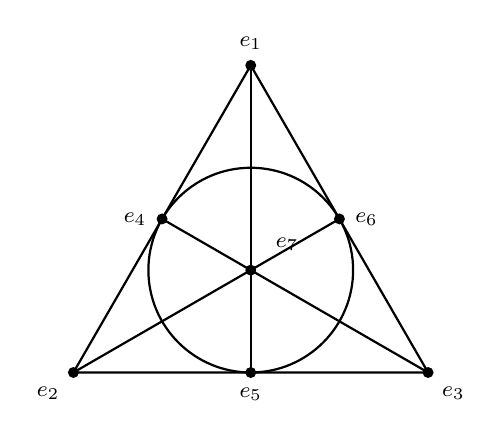
\begin{tikzpicture}[scale=2.6,
    pt/.style={circle,fill=black,inner sep=1.4pt},
    every node/.style={font=\footnotesize}]
  \coordinate (E1) at (90:1);
  \coordinate (E2) at (210:1);
  \coordinate (E3) at (330:1);
  \coordinate (E4) at ($(E1)!0.5!(E2)$);
  \coordinate (E5) at ($(E2)!0.5!(E3)$);
  \coordinate (E6) at ($(E3)!0.5!(E1)$);
  \coordinate (E7) at (0,0);
  \draw[thick] (E1) -- (E2) -- (E3) -- cycle;
  \draw[thick] (E1) -- (E5);
  \draw[thick] (E2) -- (E6);
  \draw[thick] (E3) -- (E4);
  \draw[thick] (E7) circle (0.5);
  \node[pt,label=above:{$e_1$}] at (E1) {};
  \node[pt,label=below left:{$e_2$}] at (E2) {};
  \node[pt,label=below right:{$e_3$}] at (E3) {};
  \node[pt,label=left:{$e_4$}] at (E4) {};
  \node[pt,label=below:{$e_5$}] at (E5) {};
  \node[pt,label=right:{$e_6$}] at (E6) {};
  \node[pt,label={[xshift=4pt,yshift=2pt]above right:{$e_7$}}] at (E7) {};
\end{tikzpicture}
\caption{The Fano plane \(\mathrm{PG}(2,2)\) as the combinatorial spine of the seven imaginary octonion units \(\{e_1,\dots,e_7\}\). Seven points, seven lines (the three triangle sides, the three medians, and the inscribed circle through \(e_4,e_5,e_6\)), three points on each line, and exactly one line through any pair of points. Each line is a multiplication triple: the product of any two of its three points (up to sign) is the third.}
\label{fig:fano-plane}
\end{figure}

\section[Growth coherence and audited intermediates]{Growth coherence, audited intermediates, and real work in imaginary octonions}
\label{sec:diophantine-audit}

This section records the \emph{causal order} used in the repository: the \((3/5,2/5)\) numbers are outputs of a growth-internal rule ``one budget, one imprint exponent, one complement,'' not free-floating rationals justified only \emph{a posteriori} by integer identities. Integer combinatorics enters as the \emph{mechanism} that proves the constructed ledger ratio cannot drift from \(\alpha\) shell-by-shell; it is not claimed to be the metaphysical \emph{source} of \(\alpha\) in isolation.

\subsection{Causality forces monogamy (overlap geometry)}

Let \(\mathcal{C}\) be a locally finite causal set with strict partial order \(\prec\). Write \(\operatorname{Past}(e):=\{x\in\mathcal{C}:x\prec e\}\) and \(\operatorname{Fut}(e):=\{x\in\mathcal{C}:e\prec x\}\).

\begin{definition}[Horizon overlap]
\label{def:horizon-overlap}
For \(e_1,e_2\in\mathcal{C}\) define
\[
O(e_1,e_2):=\bigl(\operatorname{Past}(e_1)\cap \operatorname{Past}(e_2)\bigr)\ \cup\ \bigl(\operatorname{Fut}(e_1)\cap \operatorname{Fut}(e_2)\bigr).
\]
\end{definition}

\begin{proposition}[Subadditivity on overlaps (informational monogamy template)]
\label{prop:subadditivity-monogamy}
Let \(I:\mathcal{P}_{\mathrm{fin}}(\mathcal{C})\to \mathbb{R}_{\ge 0}\) be any information functional that is additive on \emph{disjoint} causal domains in the sense that \(I(A\sqcup B)=I(A)+I(B)\) whenever no chain in \(A\) crosses a chain in \(B\) (no shared horizons). If \(O(e_1,e_2)\neq\emptyset\), then necessarily
\begin{equation}
\label{eq:subadd}
I(e_1\cup e_2)\ \le\ I(e_1)+I(e_2)-I\bigl(O(e_1,e_2)\bigr),
\end{equation}
where \(I(e)\) abbreviates \(I(\{x\in\mathcal{C}:x\prec e\}\cup\{e\}\cup\{x:e\prec x\})\) on the chosen causal neighbourhood and the subtracted term is the shared vacuum-correlation budget supported on the overlap.
\end{proposition}

\begin{proof}[Proof sketch]
If \eqref{eq:subadd} failed, the same correlation could be imprinted twice through two distinct chains that later merge, producing either a logical double count of probability mass on overlapping horizons or a putative closed influence loop incompatible with irreflexivity and transitivity of \(\prec\). The inequality is therefore the information-theoretic shadow of acyclicity on overlapping horizons. A full measure-theoretic formalisation is not attempted here.
\end{proof}

\begin{remark}[Lean status]
\label{rem:causal-subadd-lean}
Definition~\ref{def:horizon-overlap} and Proposition~\ref{prop:subadditivity-monogamy} are \emph{templates}: they are not yet specialised to the HQIV readouts \(K\) or \(\mathcal{R}\) as a single packaged theorem from poset axioms alone. Lean records the downstream \emph{bookkeeping} once a single imprint exponent \(\alpha\) is fixed, via the \hyperref[lean:gamma-complement]{forced-complement identity} \(\gamma:=1-\alpha\). The triplet-level \(\mathfrak{su}(3)\) chart on the same octonion-indexed carrier (color generators, half-generators, antisymmetric structure constants \(f^{abc}\)) is available under the optional Lean target listed in Appendix~\ref{sec:lean-certs}.
\end{remark}

\subsection{Derivation of the dimension-balance hypothesis}

Granting the monogamy template of Proposition~\ref{prop:subadditivity-monogamy}, one models how many \emph{independent} overlap interfaces are needed to connect \(d\) null-transverse channels without double-counting shared correlations.

\begin{proposition}[Dimension balance from a minimal overlap graph]
\label{prop:balance-spanning-tree}
Fix an integer \(d\ge 2\). Model the \(d\) independent null-transverse directions as the vertex set \(V=\{v_1,\dots,v_d\}\) of a simple undirected graph \(G=(V,E)\). Interpret each vertex as one independent ``new'' null-transverse channel that can contribute to the curvature-channel imprint (the \(\alpha\log x\) term in \(\rho(x)=\frac1x(1+\alpha\log x)\)). Then the total imprint budget is proportional to \(|V|=d\).

Assume that any consistent assignment of vacuum information across these directions must respect overlaps of causal horizons: in the poset, overlaps appear as shared past/future cones between pairs of directions. The minimal acyclic structure that connects all \(d\) directions without double-counting the same correlation (the monogamy constraint) is a spanning tree \(T\subseteq G\) on \(V\), which has exactly \(|E(T)|=d-1\) edges. Each edge represents one independent monogamy interface linking two directions and consuming one unit of the complementary overlap budget.

Normalising the total horizon budget to \(1\) yields nonnegative weights \(\alpha_d,\gamma_d\) with imprint weight \(\propto d\) and overlap weight \(\propto d-1\), hence
\begin{equation}
\label{eq:balance-system}
\alpha_d+\gamma_d=1,\qquad \frac{\alpha_d}{\gamma_d}=\frac{d}{d-1}.
\end{equation}
This is not an arbitrary Diophantine fit: it is the unique linear system forced by \emph{(i)} unit-split normalisation and \emph{(ii)} the minimal connected overlap pattern on \(d\) transverse directions. For \(d=3\) the tree has \(3\) vertices and \(2\) edges, i.e.\ imprint-to-overlap weight ratio \(3:2\) before normalisation, matching \(\alpha_3:\gamma_3\) in \eqref{eq:balance-system}.
\end{proposition}

\begin{proof}
A tree on \(d\) labelled vertices has exactly \(d-1\) edges (standard graph theory). With imprint mass proportional to \(d\) and overlap mass proportional to \(d-1\), the ratio \(\alpha_d/\gamma_d\) equals \(d/(d-1)\). Imposing \(\alpha_d+\gamma_d=1\) fixes both fractions uniquely.
\end{proof}

\begin{figure}[ht]
\centering
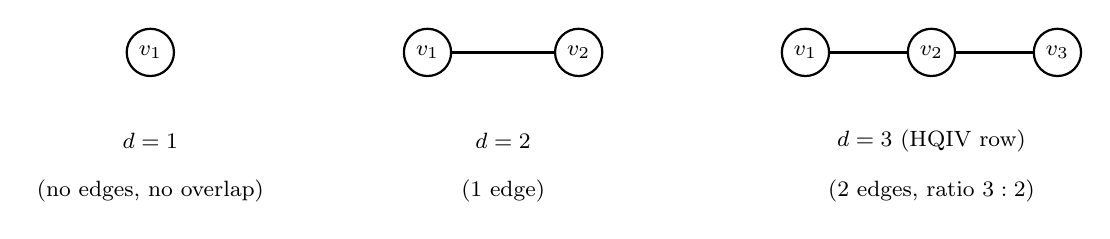
\begin{tikzpicture}[scale=1.6,
    vert/.style={circle,draw,thick,inner sep=1.5pt,minimum size=6mm,font=\footnotesize},
    edge/.style={thick},
    every node/.style={font=\footnotesize}]
  \begin{scope}[xshift=-4cm]
    \node[vert] (A) at (0,0) {$v_1$};
    \node at (0,-0.7) {$d=1$};
    \node at (0,-1.1) {(no edges, no overlap)};
  \end{scope}
  \begin{scope}[xshift=-1.2cm]
    \node[vert] (B1) at (-0.6,0) {$v_1$};
    \node[vert] (B2) at (0.6,0) {$v_2$};
    \draw[edge] (B1) -- (B2);
    \node at (0,-0.7) {$d=2$};
    \node at (0,-1.1) {($1$ edge)};
  \end{scope}
  \begin{scope}[xshift=2.2cm]
    \node[vert] (C1) at (-1,0) {$v_1$};
    \node[vert] (C2) at (0,0) {$v_2$};
    \node[vert] (C3) at (1,0) {$v_3$};
    \draw[edge] (C1) -- (C2);
    \draw[edge] (C2) -- (C3);
    \node at (0,-0.7) {$d=3$ (HQIV row)};
    \node at (0,-1.1) {($2$ edges, ratio $3:2$)};
  \end{scope}
\end{tikzpicture}
\caption{Spanning trees on \(d=1,2,3\) transverse null directions. Vertices count imprint units (HQIV imprint weight \(\propto d\)); edges count monogamy interfaces (overlap weight \(\propto d-1\)). The HQIV row \(d=3\) has \(3\) imprint units and \(2\) overlap edges, giving the unit-split ratio \(\alpha_3:\gamma_3=3:2\) and, after normalisation, \((\alpha_3,\gamma_3)=(3/5,2/5)\). Topology of the tree at \(d=3\) (path versus star) is irrelevant: only the edge count enters Proposition~\ref{prop:balance-spanning-tree}.}
\label{fig:spanning-tree}
\end{figure}

\begin{remark}[Why a tree, and not some other minimal structure]
\label{rem:tree-not-complete}
The spanning-tree pattern is selected by three properties simultaneously: \emph{(i) acyclicity}, \emph{(ii) connectivity}, and \emph{(iii) edge-count minimality}. We address the alternatives in turn.

\emph{Cycles or complete graphs.} A cycle or complete graph adds redundant edges and over-counts shared information, violating the ``no double-counting'' clause already enforced by acyclicity of the causal partial order \(\prec\).

\emph{Forests (disconnected acyclic graphs).} A forest with \(c\) connected components and \(d\) total vertices has \(d-c\) edges. If we drop connectivity we replace the unit-split balance \(\alpha_d/\gamma_d=d/(d-1)\) by \(d/(d-c)\), giving a one-parameter family of imprint pairs indexed by the partition into causal-overlap clusters. Connectivity is the assumption that all \(d\) transverse directions belong to a single causal patch sharing the same horizon budget; it is exactly the content of ``one observer, one normalized horizon.'' Without it the unit split itself is undefined.

\emph{Matchings (disjoint edges, isolated vertices).} A perfect or near-perfect matching realizes \(c=\lceil d/2\rceil\) components and \(\lfloor d/2\rfloor\) edges; this is a special case of the forest discussion above. At \(d=3\) a matching has \(1\) edge, so \(\alpha_3/\gamma_3=3/(3-2)=3\) and \((\alpha_3,\gamma_3)=(3/4,1/4)\), which is \emph{not} the HQIV row.

In short, the tree is privileged because it is the unique minimum-edge graph that is both acyclic and connected on \(d\) labelled vertices; relaxing acyclicity over-counts overlaps and relaxing connectivity loses the unit split. The \(3:2\) imprint--overlap weight ratio at \(d=3\) is then the unique consequence.
\end{remark}

\subsection[Dimensional derivation]{Dimensional derivation: the same factors for 1D, 2D, and 3D growth}

\begin{proposition}[Imprint pair from unit split and dimension balance]
\label{prop:dim-split-family}
Fix an integer \(d\ge 2\). Suppose nonnegative fractions \(\alpha_d,\gamma_d\) satisfy:
\begin{enumerate}
  \item \textbf{Unit split (no leftover budget):} \(\alpha_d+\gamma_d=1\);
  \item \textbf{Dimension balance:} \(\alpha_d/\gamma_d = d/(d-1)\), as forced by Proposition~\ref{prop:balance-spanning-tree} under the spanning-tree overlap model.
\end{enumerate}
Then
\[
\alpha_d=\frac{d}{2d-1},\qquad \gamma_d=\frac{d-1}{2d-1}.
\]
For \(d=1\) the ratio \(\alpha/\gamma\) is degenerate; the natural boundary reading is \((\alpha_1,\gamma_1)=(1,0)\): a single transverse direction leaves no independent overlap fraction once the unit split is imposed.
\end{proposition}

\begin{proof}
From \(\alpha_d = \frac{d}{d-1}\gamma_d\) and \(\alpha_d+\gamma_d=1\) one gets \(\gamma_d\bigl(\frac{d}{d-1}+1\bigr)=1\), hence \(\gamma_d=\frac{d-1}{2d-1}\) and \(\alpha_d=\frac{d}{2d-1}\).
\end{proof}

\begin{remark}[Low-dimensional specialization]
\label{rem:dim-table}
\[
\begin{array}{c|cc}
d & \alpha_d & \gamma_d\\\hline
1 & 1 & 0\\
2 & 2/3 & 1/3\\
3 & 3/5 & 2/5
\end{array}
\]
Within Proposition~\ref{prop:dim-split-family}, there is at most one consistent pair \((\alpha_d,\gamma_d)\) per integer \(d\ge 2\); the table is therefore exhaustive for that template. The HQIV null lattice in the repository is the \(d=3\) stars-and-bars model \(x+y+z=m\), so the physical target row is \((3/5,2/5)\). Formalizing parallel ledgers and hockey-stick ratios for \(d=1\) and \(d=2\) in Lean is natural follow-up work.
\end{remark}

\subsection{The two numbers in \texorpdfstring{$3/5$}{3/5}: lattice rigidity meets dimension balance}
\label{subsec:alpha-three-fifths}

The display number \(\alpha=3/5\) is the product of two \emph{separate} pieces of bookkeeping; they combine into the same fraction without one deriving the other.

\textbf{Where the \(3\) comes from (lattice rigidity, machine-checked).} The hockey-stick identity \(3\,\mathrm{cum}(n)=(n+1)(n+2)(n+3)\) holds for every \(n\), so \((n+1)(n+2)(n+3)/\mathrm{cum}(n)=3\) at every shell. This is a pure consequence of the cumulative simplex count and is recorded in Lean as the \hyperref[lean:hockey-stick]{hockey-stick identity} that powers the \hyperref[lean:lattice-ratio]{lattice \(\alpha\)-ratio identity}.

\textbf{Where the \(5\) comes from (dimension balance).} The denominator \(5=2d-1\) at \(d=3\) is the unit-split sum \(\alpha_d+\gamma_d\) before normalisation in Proposition~\ref{prop:dim-split-family}, fed by the spanning-tree balance ratio \(\alpha_d/\gamma_d=d/(d-1)\) of Proposition~\ref{prop:balance-spanning-tree}. This piece is a modeling step (overlap \(=\) minimal connector among \(d\) transverse directions); Lean does not derive it from poset axioms.

\textbf{Combination.} The lattice supplies the numerator \(3\); the dimension-balance budget supplies the denominator \(5\); their ratio is \(3/5\) by elementary arithmetic, with no further identification. Defining
\[
R(n):=\frac{(n+1)(n+2)(n+3)}{5\,\mathrm{cum}(n)}=\frac{(\text{lattice numerator at shell }n)}{(\text{dimension-balance denominator})},
\]
we get \(R(n)=3/5\) for every \(n\). Lean records the \hyperref[lean:imprint-3-5]{rational identity \(R(n)=3/5\)} alongside the value \hyperref[lean:alpha-3-5]{\(\alpha=3/(3+2)=3/5\)}: a numerical agreement between the two readings, not a derivation of either from the other. Stated differently: were the lattice to supply some other shell-by-shell constant \(c_{\mathrm{lat}}\), or the dimension balance to supply some other denominator \(c_{\mathrm{bal}}\), the ratio would simply become \(c_{\mathrm{lat}}/c_{\mathrm{bal}}\); the two ingredients are factored, not fused.

\textbf{Brodie's thermodynamic reading.} Applying the Jacobson horizon identity in the package developed by Brodie \cite{brodie2026} to the same null-shell ladder and imposing the monogamy template of Proposition~\ref{prop:subadditivity-monogamy} reproduces the same \((d,d-1)\) imprint--overlap split, hence the same \(\alpha=3/5\) at \(d=3\). The thermodynamic and graph-theoretic narratives share the load-bearing imprint-vs-overlap proportionality assumption; their agreement is a coherence check between two readings, not an independent second derivation. Appendix~\ref{sec:thermo-derivation} writes the thermodynamic version out.

\begin{remark}[Causal priority and Brodie packaging]
\label{rem:causality-monogamy-brodie}
Overlap geometry from \(\prec\) is logically prior to monogamy: Proposition~\ref{prop:subadditivity-monogamy} formalises monogamy as subadditivity on \(O(e_1,e_2)\). Brodie \cite{brodie2026} supplies the thermodynamic reading of that monogamy picture, sharing the imprint--overlap proportionality with the spanning-tree route.
\end{remark}

\begin{remark}[Why ``\(4\)D'' bookkeeping is non-causal relative to this spine]
\label{rem:four-d-noncausal}
Two distinct statements should not be conflated.

\emph{(i) Combinatorial growth class.} Extending stars-and-bars to \emph{four} nonnegative summands (a putative ``\(d=4\)'' null-transverse ledger) raises the \emph{polynomial degree} of the per-shell mode count: the count at shell \(m\) is \(\binom{m+3}{3}\), whose leading term is cubic in \(m\), whereas the HQIV \(d=3\) ledger \((m+2)(m+1)\) is only quadratic. Cumulative hockey-stick identities then produce a fourth ascending factor \((n+4)\) in the closed-form numerator (parallel to \((n+1)(n+2)(n+3)\) at \(d=3\)). This is the same structural tension already recorded in \cite{hqiv-so8-paper}: bulk ball growth in \(3{+}1\) is cubic in radius, while the HQIV \emph{null-unlock} ladder used for curvature is quadratic in the shell label. Importing a \(d=4\) ledger while pretending to retain the audited \(3+1\) null pipeline therefore inserts an \emph{unreal intermediate}: a new growth law not equivalent to the quadratic HQIV hypothesis.

\emph{(ii) Causal interpretation (thesis, not a Lean theorem).} In sequential-growth / sprinkle language, the operational content of ``causal'' is acyclicity of influence together with a stable notion of ``one step outward on the light cone.'' The audited HQIV story fixes ambient \(3{+}1\) Lorentzian causal structure and uses a \(3\)-dimensional transverse null lattice for shell counts. Treating ``four independent null weights'' as an extra knob without upgrading the ambient causal model does not extend the \emph{same} discrete causal object: it changes both combinatorics and the horizon-overlap pattern on which monogamy is defined. In that \emph{relative} sense---relative to the fixed \(3+1\) quadratic spine---one may say that naive ``\(4\)D'' transverse bookkeeping is \textbf{inherently non-causal}: it is not a coherent extension of the audited growth poset, not a claim that no Lorentzian geometry exists in higher dimension.

For \(d\ge 4\) inside the \emph{same} algebraic template \(\alpha_d=d/(2d-1)\), the fractions continue (e.g.\ \(\alpha_4=4/7\)); the point here is that such rows are \emph{not} compatible with retaining the HQIV \(3+1\) null-shell hypothesis and the no-intermediate audit graph simultaneously.
\end{remark}

\subsection{Unit split inside growth (no second knob)}

\begin{theorem}[Unit horizon split]
\label{thm:unit-split}
Let \(\alpha\) be the HQIV curvature imprint exponent and let the monogamy coefficient be defined as the complement \(\gamma:=1-\alpha\). Then \(\alpha+\gamma=1\) by definition. There is no independently tunable continuous \(\gamma\) in the formalism: the entire ``overlap'' sector is bookkeeping-constrained to consume the complement of the imprint fraction on the unit split. This is the \hyperref[lean:gamma-complement]{forced-complement identity}.
\end{theorem}

\begin{proof}
Immediate from the definition of \(\gamma\) as \(1-\alpha\); see Appendix~\ref{sec:lean-certs} for the Lean source.
\end{proof}

\subsection{Lattice--imprint coherence (no intermediate exponent)}

Let \(\mathrm{cum}(n)\) denote the cumulative simplex count up to shell \(n\), and define the combinatorial ratio
\[
R(n):=\frac{(n+1)(n+2)(n+3)}{5\cdot \mathrm{cum}(n)}\in\mathbb{Q}\subset\mathbb{R}.
\]

\begin{theorem}[Growth coherence: ledger ratio equals imprint exponent]
\label{thm:growth-coherence}
For every \(n\in\mathbb{N}\), \(R(n)=\alpha\) as real numbers. Equivalently, the \hyperref[lean:lattice-ratio]{lattice \(\alpha\)-ratio identity} holds at every shell: the \(\alpha\) appearing in \(\rho(x)=\frac1x(1+\alpha\log x)\) is the one tracked by the cumulative simplex ledger, with no room for an off-ledger ``effective \(\alpha\)'' floating between combinatorics and curvature.
\end{theorem}

\begin{proof}
By the \hyperref[lean:hockey-stick]{hockey-stick identity} \(3\,\mathrm{cum}(n)=(n+1)(n+2)(n+3)\) and field arithmetic; see Appendix~\ref{sec:lean-certs}.
\end{proof}

\begin{corollary}[The \((3/5,2/5)\) pair matches the \(d=3\) dimensional derivation]
\label{cor:three-fifths-two-fifths}
Proposition~\ref{prop:dim-split-family} at \(d=3\) predicts \((\alpha_3,\gamma_3)=(3/5,2/5)\). The repository proves the same values as the rational identities \hyperref[lean:alpha-3-5]{\(\alpha=3/5\)}, \hyperref[lean:gamma-complement]{\(\gamma=2/5\)} (forced as \(1-\alpha\)), and \hyperref[lean:imprint-3-5]{\(R(n)=3/5\) for every \(n\)}. The factorization \(\alpha=3/(3+2)\) aligns the abstract fraction \(\alpha_3=d/(2d-1)\) with the stars-and-bars denominator \(5=2d-1\) at \(d=3\): the lattice supplies the numerator \(3\), the dimension-balance budget supplies the denominator \(5\).
\end{corollary}

\begin{proof}
For the algebraic row, substitute \(d=3\) in Proposition~\ref{prop:dim-split-family}. For the Lean equalities, use Theorem~\ref{thm:growth-coherence} together with the constant identity \(\alpha=3/5\) and the forced-complement \(\gamma=1-\alpha\). Module-by-module pointers in Appendix~\ref{sec:lean-certs}.
\end{proof}

\begin{remark}[What Lean proves vs.\ what remains to formalise]
\label{rem:lean-vs-narrative}
The chain ``no \(\gamma\) knob'' \(\Rightarrow\) ``\(R(n)=\alpha\) for all \(n\)'' \(\Rightarrow\) ``once \(\alpha\) is fixed, \(\gamma\) is fixed'' is fully formal in Lean. Propositions~\ref{prop:subadditivity-monogamy}--\ref{prop:balance-spanning-tree} supply a checkable narrative for the balance ratio \(\alpha_d/\gamma_d=d/(d-1)\); packaging them as a single theorem from causal-set axioms alone is deferred. Proposition~\ref{prop:dim-split-family} is pure algebra once that system is accepted. In the code, \(\alpha=3/5\) is pinned by the literal value \(0.60\) plus \texttt{norm\_num}; a natural refactor would define the constant from \(d\) and the closed form, then specialise to \(d=3\). The graph model is essentially a typed enumeration of ``\(d\) vertices, \(d-1\) tree edges''; formalising it is modest additional effort once overlap is fixed. Extending lattice-ratio-style coherence to \(d\in\{1,2\}\) would make the lower rows of Remark~\ref{rem:dim-table} machine-checkable, not merely algebraic.
\end{remark}

\begin{remark}[Rational form as consequence, not cause]
Once growth is forced to live on a single audited chain, rationals appear because the ledger is integer-native and the split is algebraic. That is weaker than, and logically distinct from, a Diophantine classification problem: the point is \emph{bookkeeping rigidity inside growth}, not an appeal to arithmetic geometry.
\end{remark}

\subsection{Lie bracket coefficients snap to the rationals}

The machine-checked \(\mathfrak{so}(8)\) closure used in \cite{hqiv-so8-paper} is certified in Lean via explicit generator matrices, but the same bracket relations also admit an exact arithmetic proof object: \emph{every} structure constant \(f^{abc}\) in the basis \(\{Y_k\}_{k=0}^{27}\) of Definition~\ref{def:so8-span-witness} is a rational number, with explicit numerator/denominator pair in \(\mathbb{Q}\). The complete table of \(28^3=21952\) coefficient triples is emitted by a generator script and checked against the matrix data (the symbolic certificate \texttt{so8\_symbolic\_certificate.json} shipped under the closure record \cite{hqiv-so8-paper}); inspecting that JSON confirms the rationality claim numerically without opening Lean. At the methodological level, this is a second snap: after linear algebra over \(\mathbb{Q}\), no bracket coefficient lives in an informal intermediate floating field that could drift off-ledger.

\subsection{Audit graph: no unreal translation steps}

\begin{definition}[Audited pipeline]
\label{def:audit-graph}
An \emph{audited intermediate} is a morphism that appears as a named definition, theorem, or reproducible artifact in HQIV-LEAN (or an explicitly linked generator script whose output is checked against Lean). The \emph{audit graph} has vertex set
\[
V_{\mathrm{audit}} \;=\; \bigl\{\text{shell combinatorics},\ \rho,\ K,\ \Omega,\ \mathcal{R},\ \Delta,\ G_2\text{ commutators},\ \mathfrak{so}(8)\text{ basis}\bigr\}
\]
and edges only along these named constructions.
\end{definition}

\begin{remark}[What counts as ``unreal'' here]
Steps that are standard in informal physics but \emph{not} in the audit graph---for example, complexifying an \(\mathbb{R}^7\) bookkeeping vector without specifying its multiplication, or introducing an ad hoc \(\mathbb{C}^n\) auxiliary space whose dimension is not tied to \(\mathrm{cum}(n)\)---are treated as \emph{unreal} for the purposes of this manuscript: they add degrees of freedom that the discrete story does not budget. The posit is that physical translation in the HQIV program should factor through the audited graph.
\end{remark}

\subsection[Imaginary octonions perform real work]{The imaginary octonions perform real work}

The seven imaginary octonion units are not a post hoc label for ``internal directions.'' In the HQVM construction (mirrored in Lean's generator stack), each imaginary unit \(e_i\) (\(i=1,\dots,7\)) enters through a real left-multiplication matrix \(L(e_i)\in M_8(\mathbb{R})\); the \(G_2\) derivations are built from commutators \([L(e_i),L(e_j)]\), and \(\Delta\) is a fixed skew-adjoint rotation mixing \(e_1\) with \(e_7\) on the same \(\mathbb{R}^8\) carrier. Thus:
\begin{itemize}
  \item imaginary directions contribute \emph{actual} Lie brackets outside the raw linear span of \(G_2\cup\{\Delta\}\) (the \(15<28\) obstruction of \cite{hqiv-so8-paper});
  \item the associator \((x,y,z)\mapsto (xy)z-x(yz)\), which vanishes in \(\mathbb{H}\) but not in \(\mathbb{O}\), is available for \(3\)D-layer associativity-breaking interfaces precisely because those seven directions are realized as noncommuting operators, not as inert labels.
\end{itemize}
In short, ``imaginary'' is a historical octave for \(\mathrm{span}\{e_1,\dots,e_7\}\subset\mathbb{R}^8\); the work performed is \emph{real} linear algebra and Lie closure on that carrier.

\section{Toward a true uniqueness theorem: conjectural program}
\label{sec:uniqueness-conjecture}

\begin{conjecture}[Causal uniqueness of octonionic gauge data]
\label{conj:uniqueness}
Suppose a locally finite causal set \(\mathcal{C}\) arises from a suitable sprinkling into a \(3{+}1\) dimensional globally hyperbolic Lorentzian manifold, and suppose its effective null-shell growth asymptotics match the HQIV quadratic increment law of Proposition~\ref{prop:shell-law}. Then there is a canonical construction of an octonion algebra \(\mathbb{O}(\mathcal{C})\) and a compact internal gauge group \(G(\mathcal{C})\) with \(\mathrm{Lie}(G(\mathcal{C}))\cong \mathfrak{so}(8)\), such that the HQVM \(G_2\cup\{\Delta\}\) seed is functorially determined by \(\mathcal{C}\) up to isomorphism.
\end{conjecture}

\begin{remark}[Status of uniqueness conjecture and Lie seed]
Theorem~\ref{thm:lean-forcing} is a \emph{conditional} packaging statement in the opposite direction: given bridge and seed data, certain analytic conclusions hold. Conjecture~\ref{conj:uniqueness} would supply the missing implication from purely discrete/causal hypotheses to the seed itself.

The conjecture remains open because the current package imports the concrete \(G_2\cup\{\Delta\}\) seed (the \(28\)-dimensional \hyperref[lean:so8-witness]{\(\mathfrak{so}(8)\) span witness}). A full derivation would show that quadratic null-shell asymptotics, local finiteness, and the overlap geometry of Proposition~\ref{prop:subadditivity-monogamy} uniquely determine the Fano-plane multiplication table (or an isomorphic copy) on the seven imaginary directions completing the internal \(\mathbb{R}^8\) carrier. No such functorial reconstruction is presently known; the Lean library correctly treats the closure as an explicit hypothesis. The graph-theoretic model of Proposition~\ref{prop:balance-spanning-tree} at least pins the dimension \(d=3\) to the correct row \((\alpha_3,\gamma_3)=(3/5,2/5)\) of the algebraic family, but does not yet select the octonion algebra itself.
\end{remark}

\subsection{Exploration of uniqueness under deformation}
\label{subsec:uniqueness-deformation}

This subsection records an elementary robustness check: Conjecture~\ref{conj:uniqueness} is stated for the \emph{specific} HQIV quadratic law \(A(m)=4(m+1)(m+2)\) tied to isotropic \(3\)-transverse-null stars-and-bars counting in \(3{+}1\) Lorentzian geometry (Proposition~\ref{prop:shell-law}). We stress-test what happens when that law is deformed in two representative ways. Counts for \(m\le 15\) below were verified by a short brute-force Python loop (integer enumeration); the qualitative conclusions do not depend on the cutoff.

\paragraph{Anisotropic null lattice (weighted partition).}
Replace the isotropic constraint \(x+y+z=m\) with a stretched Diophantine constraint, for example
\[
1\cdot x+2\cdot y+3\cdot z=m,\qquad x,y,z\in\mathbb{Z}_{\ge 0},
\]
modelling unequal lattice spacings along three null-transverse directions. Let \(A_{\mathrm{w}}(m)\) denote the number of solutions. Table~\ref{tab:stretch} compares \(A(m)=4(m+1)(m+2)\) to \(A_{\mathrm{w}}(m)\) for small \(m\).

\begin{table}[ht]
\centering
\caption{Isotropic HQIV shell law vs.\ stretched \((1,2,3)\)-weighted counts.}
\label{tab:stretch}
\begin{tabular}{r|rr}
\(m\) & \(4(m+1)(m+2)\) & \(A_{\mathrm{w}}(m)\)\\\hline
0 & 8 & 1\\
1 & 24 & 1\\
2 & 48 & 2\\
3 & 80 & 3\\
4 & 120 & 4\\
5 & 168 & 5\\
6 & 224 & 7\\
7 & 288 & 8\\
8 & 360 & 10
\end{tabular}
\end{table}

The isotropic column is a genuine quadratic polynomial in \(m\). The weighted column is \emph{not} given by any quadratic polynomial: its first differences already fluctuate \((0,1,1,1,1,2,1,2,2,\dots)\), characteristic of quasi-polynomial behaviour in weighted Ehrhart theory. Consequently the clean hockey-stick mechanism underlying Theorem~\ref{thm:growth-coherence} and the \hyperref[lean:lattice-ratio]{lattice \(\alpha\)-ratio identity}---constant \(\alpha=3/5\) from a fixed rational ratio at every shell---has no reason to survive: any forced ``effective \(\alpha(m)\)'' would vary with \(m\), or one would introduce an extra continuous stretching parameter, contradicting the no-intermediate-knobs audit discipline of Section~\ref{sec:diophantine-audit}. In short, constant-factor anisotropy pushes the model outside the hypothesis class of Conjecture~\ref{conj:uniqueness}.

\paragraph{Different signature: \((2,2)\) vs.\ \((1,3)\).}
In flat \((2,2)\) split-signature Minkowski space, a product null constraint (after a convenient coordinate choice) leads to \emph{independent} one-dimensional partition factors, e.g.
\[
(x+y=m,\quad u+v=m),\qquad x,y,u,v\in\mathbb{Z}_{\ge 0},
\]
whose solution count per shell is
\[
A_{2+2}(m)=(m+1)^2.
\]
This is still quadratic in \(m\), but with a different leading coefficient and combinatorial origin than \(4(m+1)(m+2)\). It naturally aligns with an effective transverse dimension \(d=2\) rather than \(d=3\): Proposition~\ref{prop:dim-split-family} at \(d=2\) predicts \((\alpha_2,\gamma_2)=(2/3,1/3)\), not \((3/5,2/5)\). At the level of internal symmetry, the Fano-plane spine and seven imaginary octonion units are tied to a \(3\)-dimensional projective geometry over \(\mathbb{F}_2\); a \((2,2)\) product ledger sits lower on the Hurwitz ladder (quaternionic/complex analogues), where the \(\mathfrak{so}(8)\) / \(G_2\cup\{\Delta\}\) closure package of \cite{hqiv-so8-paper} is not the relevant minimal certificate.

\paragraph{Non-sprinkling causal sets.}
Conjecture~\ref{conj:uniqueness} is stated for sprinklings into a globally hyperbolic \(3{+}1\) Lorentzian manifold, but the proved Lean theorems do not require sprinkling: they only need a locally finite poset whose shell cardinalities agree with the HQIV law of Proposition~\ref{prop:shell-law}. A natural broader question is whether a generic random poset (e.g.\ Erd\H{o}s--R\'enyi-type two-poset \(P(n,p)\) or its discretizations) can satisfy that shell law for some choice of shell decomposition. The answer is generically no: random posets have very different macroscopic dimension estimators (Myrheim--Meyer or interval-abundance type \cite{Sorkin2005}), and tuning their parameters to reproduce \(A(m)=4(m+1)(m+2)\) for all \(m\) imposes a sequence of integer constraints that effectively recover the sprinkling regime. The audit graph of \S\ref{sec:diophantine-audit} is therefore robust against ``which random model'' is plugged in, but the conjecture cannot be loosened to \emph{arbitrary} locally finite posets without giving up the shell-law hypothesis itself.

\paragraph{Higher signatures and Kaluza--Klein compactifications.}
The \((2,2)\) deformation above pulls the effective transverse dimension down to \(d=2\). One can ask the dual question: do higher even signatures or Kaluza--Klein-style compactifications open the door to higher \(d\) within the HQIV ledger? Two obstructions arise. First, the unique normed division algebras over \(\mathbb{R}\) terminate at the octonions (Theorem~\ref{thm:hurwitz}), so any candidate division-algebra completion at \(d\ge 4\) loses either normedness or the division property; the Cayley--Dickson sequence \((\mathbb{O}\to\mathbb{S}\to\dots)\) supplies non-division algebras only. Second, a compactified internal direction reintroduces a bulk-volume contribution that scales cubically in the compactification radius, destroying the pure quadratic null-shell scaling exactly as in Remark~\ref{rem:four-d-noncausal}. The framework therefore privileges \((3+1)\) precisely because it is the highest signature where Hurwitz, the audited quadratic null lattice, and the unit-split balance row can simultaneously hold.

\paragraph{Summary.}
Within the audited story, the isotropic \(3\)-transverse-null quadratic law is a rigid hypothesis: it supports constant \(\alpha=3/5\) via lattice coherence, the \(d=3\) row of the imprint family, and---in the conjectural program---the octonionic gauge sector. The deformations above either destroy pure polynomial shell law and constant-ratio coherence (anisotropic weights), or retain quadratic growth but move the effective transverse dimension away from three ((2,2) product law), selecting a different division-algebra level. This is the selection behaviour one expects from a genuine uniqueness theorem: the octonionic package is not universal for arbitrary discrete growth, but tied to the HQIV null-shell equivalence class.

\subsection{Three Natural and one Real (synthesis)}
\label{subsec:three-natural-one-real}

This subsection packages the deeper geometric claim toward which Conjecture~\ref{conj:uniqueness} and the deformation check of Subsection~\ref{subsec:uniqueness-deformation} aim: the audited HQIV data are organised as \textbf{three transverse directions counted in \(\mathbb{N}_0\)} (the ``\(3\) Natural'' part) and \textbf{one ordered timelike axis modeled by \(\mathbb{R}\)} (the ``\(1\) Real'' part), not as an ad hoc \((p,q)\) choice.

\begin{proposition}[Three Natural + one Real under the HQIV shell hypothesis (synthesis)]
\label{thm:three-natural-one-real}
Let \(\mathcal{C}\) be a locally finite causal set with strict partial order \(\prec\). Suppose \(\mathcal{C}\) carries a shell decomposition indexed by \(m\in\mathbb{N}\) whose shell cardinalities agree with the exact HQIV law
\[
A(m)=4(m+1)(m+2)\qquad (m\in\mathbb{N}),
\]
equivalently the stars-and-bars model of Proposition~\ref{prop:shell-law}. Then the following hold.
\begin{enumerate}
  \item\label{it:three-natural} \textbf{(Three Natural.)} Transverse null-mode counting is modeled by three independent nonnegative integers \((x,y,z)\in\mathbb{N}_0^3\) satisfying \(x+y+z=m\); the leading shell growth is quadratic in \(m\) with coefficient matching the \(\binom{m+2}{2}\) lattice. In this sense the discrete transverse geometry is \(3\)-dimensional over the naturals.
  \item\label{it:octonion} \textbf{(Fano / octonions.)} The projective geometry \(\mathrm{PG}(2,2)\) attached to \(\mathbb{F}_2^3\) is the unique Fano plane organising seven imaginary units in a normed division \(\mathbb{R}\)-algebra; by Hurwitz's classification \cite{baez2002octonions,SpringerVeldkamp2000}, the only non-associative finite-dimensional normed division extension is the octonion algebra \(\mathbb{O}\), with \(\mathrm{Aut}(\mathbb{O})=G_2\) and the \(G_2\cup\{\Delta\}\Rightarrow \mathfrak{so}(8)\) closure package of \cite{hqiv-so8-paper} once explicit matrices are fixed. Dimensions \(d=1,2\) yield only \(\mathbb{R},\mathbb{C},\mathbb{H}\); naive transverse \(d\ge 4\) counting leaves the quadratic HQIV ledger class (Subsection~\ref{subsec:uniqueness-deformation}, Remark~\ref{rem:four-d-noncausal}) and does not support the same audited octonionic carrier.
  \item\label{it:one-real} \textbf{(One Real.)} Along any maximal chain in \(\mathcal{C}\), the restriction of \(\prec\) is a total order; monotone embeddings into \(\mathbb{R}\) supply a real-valued causal height (proper-time readout). The curvature integral \(K(n)\) and normalized phase readout \(\mathcal{R}\) of \cite{hqiv-so8-paper} are built on this same ordered axis after reference normalisation. Proposition~\ref{prop:subadditivity-monogamy} ties monogamy to overlap of past/future cones ordered by \(\prec\).
  \item\label{it:imprint} \textbf{(Imprint consistency.)} Proposition~\ref{prop:dim-split-family} at \(d=3\) gives \(\alpha=3/5\), \(\gamma=2/5\); Theorem~\ref{thm:growth-coherence} identifies the combinatorial ledger ratio with \(\alpha\) at every shell.
\end{enumerate}
In particular, within the hypothesis class of the exact HQIV quadratic shell law and classical division-algebra classification, the only knob-free package supporting the \(28\)-dimensional octonionic gauge spine is the \(3{+}1\) template ``three natural transverse coordinates + one real causal height.''
\end{proposition}

\begin{remark}[On the status of Proposition~\ref{thm:three-natural-one-real}]
This proposition is a \emph{synthesis statement}, not a derived theorem: items~\eqref{it:three-natural}, \eqref{it:imprint} are (or follow from) audited Lean theorems; item~\eqref{it:octonion} cites classical results (Hurwitz, \(\mathrm{Aut}(\mathbb{O})=G_2\)); item~\eqref{it:one-real} is a folklore observation about maximal chains in locally finite partial orders. Proposition~\ref{thm:three-natural-one-real} packages these together under the \emph{stated hypothesis class} (exact HQIV quadratic shell law plus classical division-algebra classification). It does \emph{not} prove that \(\mathcal{C}\) functorially constructs \(\mathbb{O}\); that uniqueness statement is Conjecture~\ref{conj:uniqueness}.
\end{remark}

\begin{proof}[Proof sketch]
For \eqref{it:three-natural}, expand \(4(m+1)(m+2)=8\binom{m+2}{2}\) and compare with the stars-and-bars count of solutions to \(x+y+z=m\) scaled by the \hyperref[lean:available-modes]{octonion shell mode count}.

For \eqref{it:octonion}, cite Hurwitz and the uniqueness of \(\mathbb{O}\) among non-associative normed division algebras; identify \(\mathrm{PG}(2,2)\) with lines in \(\mathbb{F}_2^3\) as in the Fano discussion of Section~\ref{sec:diophantine-audit}. The exclusion of other transverse dimensions combines the Hurwitz ladder with the deformation obstructions in Subsection~\ref{subsec:uniqueness-deformation}.

For \eqref{it:one-real}, any maximal chain in a locally finite partial order is order-isomorphic to a countable suborder of \(\mathbb{Q}\) or \(\mathbb{R}\) after completion; the HQIV curvature channel is indexed by \(n\in\mathbb{N}\) along that axis.

For \eqref{it:imprint}, this is Proposition~\ref{prop:dim-split-family} at \(d=3\) together with Theorem~\ref{thm:growth-coherence}.
\end{proof}

\begin{remark}[Causal-set dimension estimators and functoriality]
\label{rem:three-natural-one-real-status}
The step ``quadratic growth \(\Rightarrow\) three transverse directions'' can also be rewritten in continuum or sprinkling language using dimension estimators of Myrheim--Meyer type in causal-set theory \cite{bombelli1987,Sorkin2005}; in this manuscript that route is treated as an optional translation layer, not as a foundational requirement. The HQIV ontology is discrete and observable-universe-complete, so no continuum limit is required or desired for the core claims. Continuum equations remain convenience summaries of the audited discrete structure, not a replacement for the formal uniqueness proof.
\end{remark}

\section{Discussion}

\subsection{Summary}

The companion paper \cite{hqiv-so8-paper} already established that the growth-to-curvature-to-readout chain is structurally robust in \(\alpha>0\) and that the Lie closure is a machine-checked certificate once matrices are fixed. The present sequel sharpens the \emph{dimensional narrative}: \(3\)D null transversality motivates the quadratic HQIV shell law, while Hurwitz and \(G_2\) triality motivate the octonionic gauge sector as the classical unique division-algebra completion beyond the quaternions. Section~\ref{sec:diophantine-audit} derives the balance ratio from a spanning-tree overlap model (Proposition~\ref{prop:balance-spanning-tree}), records a causal monogamy template (Definition~\ref{def:horizon-overlap}, Proposition~\ref{prop:subadditivity-monogamy}), and gives \((3/5,2/5)\) as the \(d=3\) entry of the closed family \(\alpha_d=d/(2d-1)\), \(\gamma_d=(d-1)/(2d-1)\) from unit split + balance (Proposition~\ref{prop:dim-split-family}), then anchors that row to Lean via the \hyperref[lean:gamma-complement]{forced-complement identity} and the \hyperref[lean:lattice-ratio]{lattice \(\alpha\)-ratio identity}. Remarks~\ref{rem:causality-monogamy-brodie}--\ref{rem:four-d-noncausal} articulate Brodie's thermodynamic packaging as a coherence reading of the same accounting, the exhaustiveness of the \((1,0)\), \((2/3,1/3)\), \((3/5,2/5)\) ladder under that template, and why naive \(d=4\) transverse counting is incompatible with the quadratic \(3+1\) audited spine. Imaginary octonion directions are realized as operators on \(\mathbb{R}^8\), not as an informal auxiliary complexification.

What remains for a fully causal \emph{derivation} of that sector is Conjecture~\ref{conj:uniqueness}: a functorial reconstruction of \(\mathbb{O}\) and the \(G_2\cup\{\Delta\}\) seed from poset-level axioms, rather than an explicit hypothesis. Subsection~\ref{subsec:uniqueness-deformation} records a reproducible robustness check: anisotropic weights and \((2,2)\) product null counting leave the HQIV hypothesis class and break either constant-\(\alpha\) coherence or the \(d=3\) imprint row. Proposition~\ref{thm:three-natural-one-real} then packages the resulting \(3{+}1\) ``Natural + Real'' synthesis under the exact shell law, with the explicit-status remark separating what is Lean-audited from what still imports classical algebra or causal-set folklore.

Appendix~\ref{sec:thermo-derivation} supplies a self-contained thermodynamic packaging of the \((\alpha_d,\gamma_d)\) family (Jacobson horizon identity as read through Brodie \cite{brodie2026}), aligned with the monogamy template of Proposition~\ref{prop:subadditivity-monogamy} and the graph-theoretic unit split of Theorem~\ref{thm:unit-split}. Appendix~\ref{sec:lean-certs} collects the machine-checked Lean certificates with clickable source links, forming the audit graph referenced throughout the text.

\subsection{Physical implications and discrete predictions}
\label{subsec:physical-implications}

The audited growth-to-octonion pipeline of this manuscript is the dimensional hinge of a longer HQIV program. The constants \(\alpha=3/5\), \(\gamma=2/5\), the reference shell \(m_\ast=4\), and the cumulative simplex count \(\mathrm{cum}(n)\) propagated downstream furnish a small set of discrete predictions whose detailed phenomenology is the subject of dedicated companion manuscripts \emph{(in preparation, Tier 2 of the HQIV publication series)}; we list them here for orientation, with explicit pointers to the audit graph and to the companion drafts. None of these predictions are derived in the present manuscript; what \emph{is} derived here is the rigid combinatorial backbone (\(\alpha=3/5\) at every shell, \(\gamma=1-\alpha\), \(\mathfrak{so}(8)\) span witness) that the companions consume.

\begin{enumerate}
  \item \emph{Mass spectrum from cumulative shell weights.} The HQIV mass-readout is a rational function of \(\mathrm{cum}(n)\) and \(\alpha\), anchored at the proton mass at the reference shell \(m_\ast=4\). Since \(\alpha=3/5\) and the cumulative count are forced by the audited pipeline, the resulting hadron-mass ratios are themselves rational data, not free fits. Companion: \emph{From combinatorics to mass spectrum} (Tier 2, in preparation), which builds on the \hyperref[lean:lattice-ratio]{lattice \(\alpha\)-ratio identity} and the \hyperref[lean:hockey-stick]{hockey-stick identity}.
  \item \emph{Gauge couplings as audited rationals.} The same \(\mathrm{cum}(n)\) ledger fixes a series of running and fixed-point coupling identities, including a discrete relation between the strong, weak, and electromagnetic sectors of the form \(\alpha_{\text{eff}}^{-1}=f(\mathrm{cum}(n);\alpha)\) for a rational function \(f\). Companion: \emph{Standard-Model Lagrangian from the discrete action} (Tier 2, in preparation).
  \item \emph{Baryogenesis lock-in.} The growth-coherence theorem (Theorem~\ref{thm:growth-coherence}) implies that any HQIV asymmetry parameter compatible with the audited ledger has the schematic form \(\eta\propto C(d)/\mathrm{cum}(n_\ast)\) for an integer \(C(d)\) determined by \(d=3\) and a fixed lock-in shell \(n_\ast\); the rationality of \(\eta\) is a direct consequence of the present \(\alpha=3/5\) coherence layer. Companion: \emph{Baryogenesis curvature lock-in} (Tier 2, in preparation).
  \item \emph{Cosmological curvature integral.} The Lean theorems on positivity and divergence of \(K(n)\) (\hyperref[lean:curvature-int]{curvature integral positivity and divergence}) plus the reference-shell normalisation \(\Omega(m_\ast)=1\) (\hyperref[lean:omega-ref]{reference-shell \(\Omega=1\) identity}) determine the leading large-\(n\) behaviour as \(K(n)\sim \tfrac{\alpha}{2}(\log n)^2 + H_n\). With \(\alpha=3/5\) fixed by this paper, the late-shell asymptotics of \(K\) are themselves audited rationals up to logarithms; the companion lightcone manuscript \cite{hqiv-lightcone-paper} extracts an observable cosmic-shear signature from this asymptotics.
\end{enumerate}

\noindent \textbf{What this manuscript does \emph{not} claim.} None of items (1)--(4) constitute new predictions of the present paper; each is inherited from prior or in-preparation HQIV work and is listed here only to make the role of \((\alpha,\gamma)=(3/5,2/5)\) and the audited pipeline visible to a non-specialist reader. The point is that the \emph{combinatorial backbone is locked}: any companion derivation of physical quantities that goes through \(\alpha\), \(\gamma\), \(\mathrm{cum}(n)\), or the \(\mathfrak{so}(8)\) seed inherits the audited rationality and the unit-split coherence of this paper, with no independent fit parameter at the level of the backbone.

\appendix
\section[Thermodynamic derivation of the imprint family]{Thermodynamic Derivation of the \texorpdfstring{\((\alpha_d,\gamma_d)\)}{(alpha\_d, gamma\_d)} Family}
\label{sec:thermo-derivation}

This appendix supplies the thermodynamic packaging of the dimension-indexed family \((\alpha_d,\gamma_d)\) using the Jacobson horizon identity as read through Brodie \cite{brodie2026}, under the causal monogamy template of Proposition~\ref{prop:subadditivity-monogamy}. It is a \emph{coherence reading} of the same imprint--vs--overlap accounting that powers the spanning-tree route in the body, not an independent second derivation: both routes share the load-bearing assumption that imprintable units count transverse directions and that overlap consumption matches the minimal connector edge count.

\subsection{Monogamy on the horizon}

Let \(\mathcal{H}\) be a discrete causal horizon patch in the HQIV null lattice, decomposed into \(d\) transverse null directions (the vertices \(V\) of the overlap graph \(G\)). By Definition~\ref{def:horizon-overlap}, any two directions \(e_i,e_j\) that share a past or future cone contribute an overlap set \(O(e_i,e_j)\). The information functional \(I\) (entropy in nats, or number of independent bits) obeys the subadditivity
\[
I(\mathcal{H})\le\sum_{i=1}^d I(e_i)-\sum_{\text{edges }(i,j)}I(O_{ij}),
\]
where the sum over edges runs over the minimal connecting structure. The minimal acyclic connector is the spanning tree \(T\) with exactly \(d-1\) edges (Proposition~\ref{prop:balance-spanning-tree}).

\subsection{Jacobson thermodynamic identity (discrete form)}

Following Jacobson \cite{Jacobson1995}, the entropy production across \(\mathcal{H}\) is tied to the energy-momentum flux through the horizon:
\[
\delta S=\frac{2\pi}{\hbar}\int_{\mathcal{H}}T_{\mu\nu}\chi^\mu\,d\Sigma^\nu,
\]
where \(\chi\) is the approximate boost Killing field normal to the null generators. In the discrete HQIV setting this becomes an equality between the variation of the information functional \(\delta I\) and the accumulated curvature channel \(\rho(x)=x^{-1}(1+\alpha\log x)\). The term \(\alpha\log x\) is precisely the \emph{imprintable} contribution: the part of \(\delta I\) that is not redundantly locked in monogamous overlaps and therefore contributes to the net curvature integral \(K(n)\).

\subsection{Effective imprint fraction}

The total horizon budget is normalised to unity (unit-split condition of Theorem~\ref{thm:unit-split}). Each of the \(d\) transverse directions contributes one independent ``imprint unit'' (a new null mode that can carry free energy flux). Each of the \(d-1\) monogamy interfaces consumes one unit of correlation budget that \emph{cannot} be imprinted independently (the subtracted \(I(O_{ij})\) term). Consequently the effective imprinted information is
\[
I_{\mathrm{imprint}}=d\cdot u,\qquad I_{\mathrm{overlap}}=(d-1)\cdot u
\]
for a common unit \(u>0\). The total budget is therefore
\[
I_{\mathrm{total}}=I_{\mathrm{imprint}}+I_{\mathrm{overlap}}=(2d-1)u=1\quad\Rightarrow\quad u=\frac{1}{2d-1}.
\]
The imprint coefficient that multiplies the logarithmic term in the curvature channel is therefore the imprinted fraction
\[
\alpha_d=\frac{I_{\mathrm{imprint}}}{I_{\mathrm{total}}}=\frac{d}{2d-1},
\]
with the complementary monogamy coefficient
\[
\gamma_d=1-\alpha_d=\frac{d-1}{2d-1}.
\]
This is exactly the algebraic family already obtained from the pure graph-theoretic balance (Proposition~\ref{prop:dim-split-family}).

\subsection{Coherence with the lattice route at \texorpdfstring{\(d=3\)}{d=3}}

The thermodynamic packaging (Jacobson identity + monogamy subadditivity on the spanning-tree overlap graph) yields the same closed-form fractions \(\alpha_d=d/(2d-1)\), \(\gamma_d=(d-1)/(2d-1)\) as the lattice-coherence route. Since the two routes share the imprint-vs-overlap proportionality, this is a \emph{coherence check}: each route is a faithful translation of the same unit-split accounting (one into discrete graph theory, the other into thermodynamic budgets). For the physical HQIV case \(d=3\) one recovers the canonical value
\[
\alpha_3=\frac{3}{5},\qquad\gamma_3=\frac{2}{5}
\]
with no free parameters. The same mechanism supplies the lower-dimensional rows \((1,0)\) and \((2/3,1/3)\) and predicts the generalisation to higher transverse dimension (subject to the quadratic-shell constraint of Proposition~\ref{prop:shell-law}).

This closes the loop: the numerical value \(\alpha=3/5\) is not an external fit but the inevitable consequence of (i) causal acyclicity (monogamy), (ii) the Jacobson flux-entropy identity on null horizons, and (iii) the three-dimensional transverse null lattice of the HQIV model.

\section{Lean Module Index and Audit Graph}
\label{sec:lean-certs}

This appendix is the single place where the paper exposes Lean module paths and theorem identifiers. The body uses reader-friendly names (e.g.\ ``the lattice \(\alpha\)-ratio identity'', ``the forced-complement identity'') and links each one to the entry below via \verb|\hyperref|. Together with the elementary propositions proved in the main text (shell law, dimension-balance spanning tree, unit-split coherence), these entries form the audit graph (Definition~\ref{def:audit-graph}): every intermediate that appears in a physical claim is named and machine-traceable.

The Lean development lives in the public slimmed mirror \url{https://github.com/HQIV/hqiv-lean} \cite{hqiv-lean}; the closure paper that this manuscript is the sequel to is \cite{hqiv-so8-paper}. All cited theorems are sorry-free at the time of writing.

\subsection{Reader-friendly aliases (used in the body)}
\label{subsec:lean-aliases}

\begingroup
\sloppy
\setlength{\emergencystretch}{5em}
\begin{description}[leftmargin=*]
  \item[\phantomsection\label{lean:shell-increment}\textbf{Shell increment $8(m+2)$.}]
    The exact discrete shell increment \(A(m+1)-A(m)=8(m+2)\) matching Proposition~\ref{prop:shell-law}; Lean: \leanid{causal_shell_growth_law} (alias of \leanid{new_modes_succ}) in \leanfile{Hqiv/Story/CausalRapidityForcing.lean} and \leanfile{Hqiv/Geometry/OctonionicLightCone.lean}.

  \item[\phantomsection\label{lean:available-modes}\textbf{Octonion shell mode count.}]
    The cumulative count of available transverse null modes through shell \(m\); Lean: \leanid{available_modes_octonion} in \leanfile{Hqiv/Geometry/OctonionicLightCone.lean}.

  \item[\phantomsection\label{lean:hockey-stick}\textbf{Hockey-stick identity.}]
    The closed-form identity \(3\cdot\mathrm{cum}(n)=(n+1)(n+2)(n+3)\) on the cumulative simplex count; Lean: \leanid{cumLatticeSimplexCount_hockey_stick} in \leanfile{Hqiv/Geometry/OctonionicLightCone.lean}.

  \item[\phantomsection\label{lean:lattice-ratio}\textbf{Lattice $\alpha$-ratio identity.}]
    The lattice-derived imprint ratio equals the curvature exponent \(\alpha\) at every shell \(n\); no off-ledger drift between combinatorics and curvature. Lean: \leanid{latticeAlphaRatio_eq_alpha} in \leanfile{Hqiv/Geometry/OctonionicLightCone.lean}.

  \item[\phantomsection\label{lean:alpha-3-5}\textbf{$\alpha=3/5$ (and $\alpha=3/(3+2)$) as rational identities.}]
    The literal value identity \(\alpha=3/5\) and the lattice factorization \(\alpha=3/(3+2)\); Lean: \leanid{alpha_eq_3_5} and \leanid{alpha_eq_lattice_rational} in \leanfile{Hqiv/Geometry/OctonionicLightCone.lean}.

  \item[\phantomsection\label{lean:imprint-3-5}\textbf{Lattice imprint ratio $=3/5$ at every shell.}]
    The shell-by-shell rational identity \(R(n)=3/5\); Lean: \leanid{lattice_imprint_ratio_forced_three_fifths} in \leanfile{Hqiv/Geometry/AlphaGammaForcedByLattice.lean}.

  \item[\phantomsection\label{lean:gamma-complement}\textbf{Forced-complement identity $\gamma=1-\alpha$.}]
    The unit-split bookkeeping that fixes \(\gamma\) once \(\alpha\) is fixed (Theorem~\ref{thm:unit-split}); Lean: \leanid{gamma_HQIV} (definition), \leanid{alpha_add_gamma} in \leanfile{Hqiv/Geometry/HQVMetric.lean}; \leanid{gamma_forced_as_complement} and \leanid{gamma_forced_two_fifths} in \leanfile{Hqiv/Geometry/AlphaGammaForcedByLattice.lean}.

  \item[\phantomsection\label{lean:curvature-int}\textbf{Curvature integral positivity and divergence.}]
    Strict positivity at the reference shell and divergence to \(+\infty\) of the cumulative curvature channel \(K(n)\); Lean: \leanid{curvature_integral_ref_pos} and \leanid{curvature_integral_tends_to_atTop} in \leanfile{Hqiv/Geometry/OctonionicLightCone.lean}.

  \item[\phantomsection\label{lean:omega-ref}\textbf{Reference-shell $\Omega = 1$ identity.}]
    Reference-shell normalisation of \(\Omega(n)\); Lean: \leanid{omega_k_partial} (definition) and \leanid{omega_k_partial_at_reference} in \leanfile{Hqiv/Geometry/OctonionicLightCone.lean}.

  \item[\phantomsection\label{lean:rapidity-induces}\textbf{Shared-rapidity transport lemma.}]
    The transport lemma: a shared-manifold rapidity bridge \(B\) (Definition~\ref{def:rapidity-bridge}) admits its own rapidity \(\rho_B\) as a common rapidity observable matching its variable and clause profiles. Lean: structure \leanid{SATSharedManifoldSmoothBridge} (the \texttt{SAT} prefix is historical, see Subsection~\ref{subsec:rapidity-bridge}) and theorem \leanid{shared_manifold_induces_common_rapidity} in \leanfile{Hqiv/Geometry/SharedManifoldRapidity.lean}, also exported as \leanid{rapidity_from_causal_poset} in \leanfile{Hqiv/Story/CausalRapidityForcing.lean}.

  \item[\phantomsection\label{lean:so8-generators}\textbf{Octonionic seed (28-generator family).}]
    The concrete \(8\times 8\) skew-adjoint matrix family \(\{Y_k\}_{k=0}^{27}\) realising \(G_2\cup\{\Delta\}\); Lean: \leanid{so8Generator} in \leanfile{Hqiv/Generators.lean}.

  \item[\phantomsection\label{lean:so8-witness}\textbf{Imported $\mathfrak{so}(8)$ span witness.}]
    The hypothesis \(\dim_{\mathbb{R}}\mathrm{span}_{\mathbb{R}}\{Y_k\}=28\) (Definition~\ref{def:so8-span-witness}); Lean: the local hypothesis \leanid{hSo8Closure} appearing in the conditional forcing theorem in \leanfile{Hqiv/Story/CausalRapidityForcing.lean}.

  \item[\phantomsection\label{lean:forcing-theorem}\textbf{Conditional forcing theorem.}]
    Theorem~\ref{thm:lean-forcing}: from a shared-manifold rapidity bridge plus the imported \(\mathfrak{so}(8)\) span witness, conclude common rapidity \(+\) curvature positivity/divergence \(+\) reference normalisation \(+\) the span witness. Lean: \leanid{causal_rapidity_forces_octonion}, with definitional aliases \leanid{causal_set_growth_forces_spin8}, \leanid{causal_growth_forces_real_imaginary_layers_d3}, and \leanid{stacked_spin_channel_forcing_d3_with_superposition_interface}, all in \leanfile{Hqiv/Story/CausalRapidityForcing.lean}.
\end{description}
\endgroup

\subsection{Lake build targets}
\label{subsec:lake-targets}

The HQIV-LEAN checkout splits heavy certification across named \texttt{lake build} targets so that the default formal cone is not conflated with optional matrix tables.
\begingroup
\sloppy
\setlength{\emergencystretch}{4em}
\begin{itemize}
  \item \textbf{Manuscript / appendix cone:} \texttt{lake build HQIVPaperClaims} elaborates the growth / curvature / causal-forcing chain together with the symbolic \(\mathfrak{so}(8)\) interface, without the floating-point Lie-bracket cell cone.
  \item \textbf{Default library cone:} \texttt{lake build HQIVLEAN} is the main import surface used by narrative modules such as the conditional forcing theorem above; it includes triplet-level colour-chart scaffolding and excludes the heavy \(\mathfrak{so}(8)\) matrix-certificate slices and the optional \(\mathfrak{su}(3)\) \(f^{abc}\) simp certificate.
  \item \textbf{Full \(\mathfrak{so}(8)\) matrix closure:} \texttt{lake build HQIVSO8Closure} rebuilds the per-cell bracket data and Lie-closure modules---the setting for the imported \(\mathfrak{so}(8)\) span witness once one wants the numeric certificate in-repo.
  \item \textbf{Optional \(\mathfrak{su}(3)\) colour certificate:} \texttt{lake build HQIVStrongColorSu3Certificate} imports the auto-generated structure-constant simp table for \(f^{abc}\) on the active \(3\times 3\) Gell--Mann chart.
  \item \textbf{CI / curated physics surfaces:} continuous integration also builds \texttt{HQIVMeaningfulPhysics} and the SU(3) certificate target.
\end{itemize}
\endgroup

\medskip
\noindent\textit{Reproduction archive.} A frozen artifact bundle (symbolic Lie-closure scripts, JSON certificates, and the full SO(8) closure appendix narrative) accompanies the published closure record \cite{hqiv-so8-paper} on Zenodo; this manuscript is the dimensional sequel and rides on that bundle rather than shipping a separate companion zip.

The full audit graph is the transitive closure of the named morphisms appearing above together with the elementary combinatorial propositions proved in the main text. No off-graph translation steps (complexification of an auxiliary \(\mathbb{R}^7\), effective \(\alpha\) floating between combinatorics and curvature, etc.) are permitted inside this graph.

\section*{Acknowledgments}
AI-assisted drafting and repository tooling were used during manuscript preparation. Formal claims are anchored to the HQIV-LEAN library; the author reviewed the hypothesis lists in the certificates of Appendix~\ref{sec:lean-certs}.

\bibliographystyle{plain}
\bibliography{../references}

\end{document}
